This chapter reports the experimental results of the five 3D architectures on the ADNI cohort, under the strict subject-level five-fold protocol defined in Chapter~\ref{cha:MethodologyAndImplementationU}. Results are presented for the headline binary CN-vs-AD task and the harder three-class CN/MCI/AD benchmark, followed by an analysis of the single-vs-hybrid question, the effect of medical transfer learning, the behaviour of the transformer models, and an explainability study. All numbers are mean $\pm$ standard deviation across the five subject-disjoint folds (population standard deviation, $\mathrm{ddof}=0$), with macro-F1 as the primary metric. Every result should be read against the majority-class baseline of always predicting CN ($65.4\%$ binary, $52.2\%$ three-class accuracy), which is included in the main tables.

\section{Experimental Setup Recap}
Every model was trained and evaluated on the \emph{same} folds (\texttt{seed = 42}), with the same preprocessing, classifier head, imbalance handling, and evaluation; the backbone and its schedule differ (Appendix~\ref{app:repro}). Predictions are aggregated to the subject level by averaging a subject's per-scan softmax probabilities. Because CN is the majority class and MCI the minority, accuracy alone is misleading, so macro-F1 (the unweighted mean of per-class F1) is treated as the headline number and drives model selection and early stopping.

\section{Binary CN-vs-AD Results (Headline)}
Table~\ref{tab:binary} reports the binary task. The proposed \textbf{hybrid 3D CNN--ViT} has the highest mean at $82.2\%$ accuracy and $0.802$ macro-F1, but the from-scratch 3D DenseNet CNN ($81.0\%$, $0.788$) is statistically indistinguishable from it (Section~\ref{sec:rq1}). Both clear the $65.4\%$ majority-class baseline by a wide margin. The Swin+ViT hybrid and the MedicalNet-pretrained ResNet trail by roughly 12 points, sit only about 4--5 points above the majority baseline in accuracy, and show markedly higher variance across folds. Standalone ViT and Swin models were not run on the binary task.

\begin{table}[H]
\centering
\caption{Binary CN-vs-AD, subject-level 5-fold cross-validation (mean $\pm$ std).}
\label{tab:binary}
\begin{tabular}{|l|c|c|c|}
\hline
\textbf{Model} & \textbf{Accuracy} & \textbf{Macro-F1} & \textbf{Weighted-F1} \\
\hline
\textbf{Hybrid 3D CNN--ViT (concat)} & \textbf{0.822 $\pm$ 0.057} & \textbf{0.802 $\pm$ 0.062} & \textbf{0.820} \\
3D CNN (DenseNet-121, scratch) & 0.810 $\pm$ 0.041 & 0.788 $\pm$ 0.062 & 0.807 \\
Hybrid Swin--ViT & 0.702 $\pm$ 0.070 & 0.662 $\pm$ 0.101 & 0.696 \\
3D ResNet (MedicalNet pretrained) & 0.698 $\pm$ 0.139 & 0.654 $\pm$ 0.168 & 0.678 \\
\hline
\textit{Majority-class baseline (always CN)} & \textit{0.654} & \textit{0.395} & \textit{0.517} \\
\hline
\end{tabular}
\end{table}

\begin{figure}[H]
    \centering
    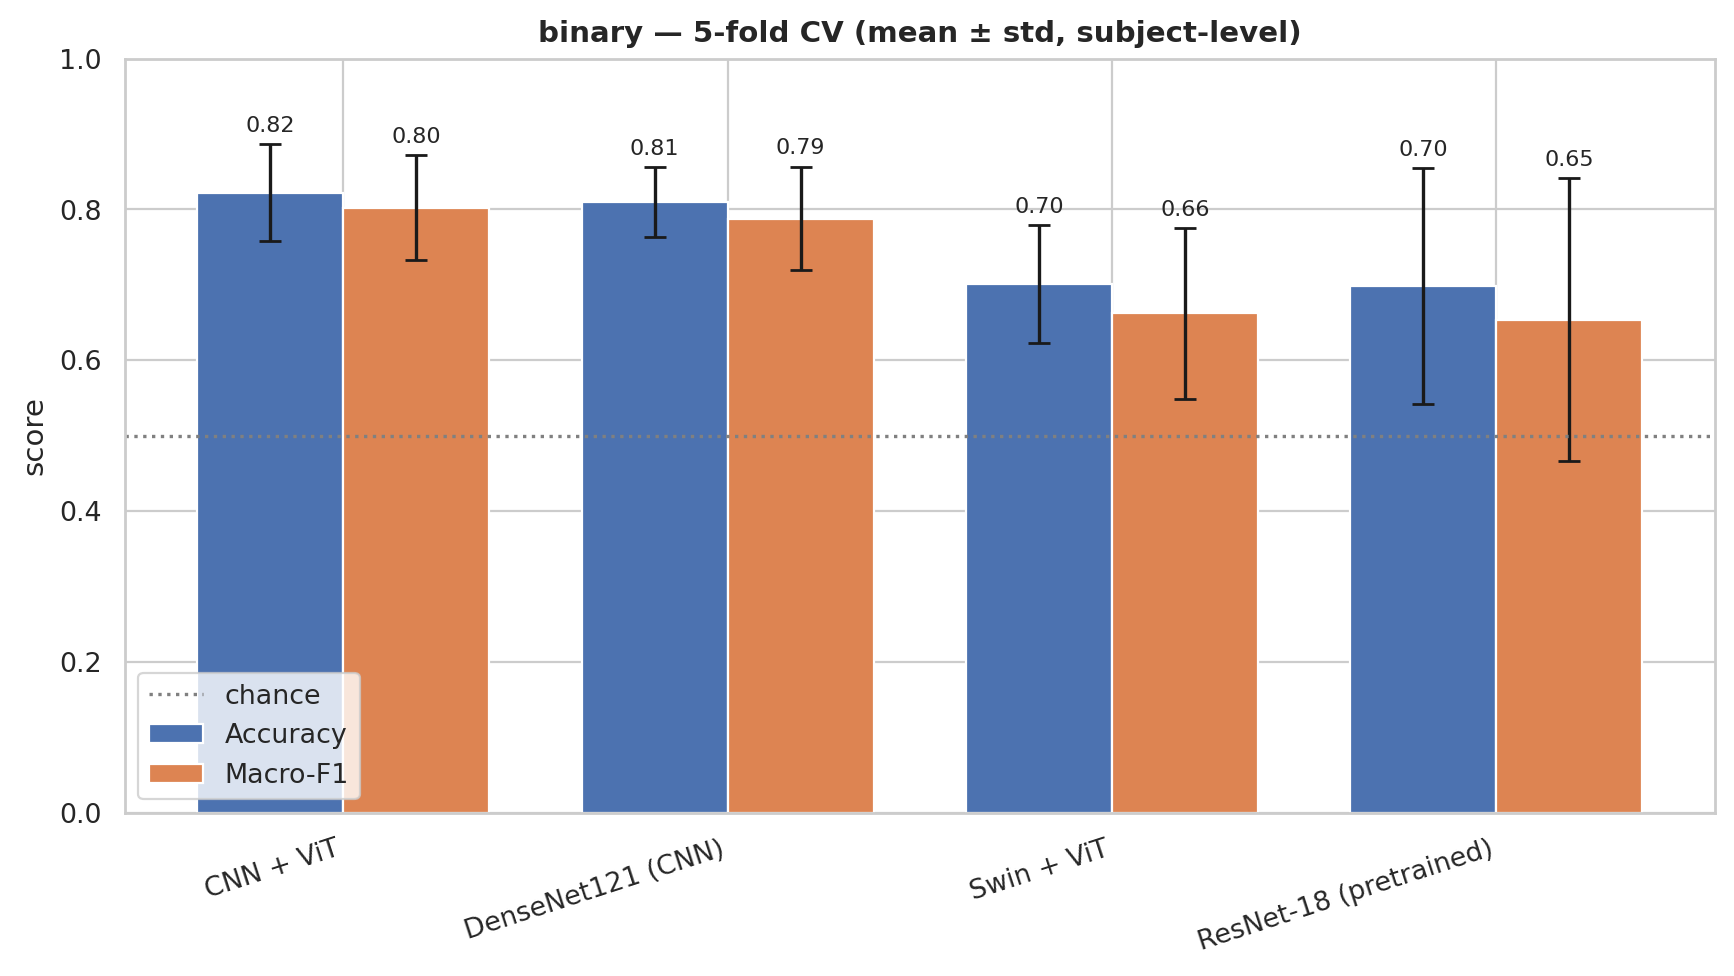
\includegraphics[width=14cm]{Images/res_bar_binary.png}
    \caption[Binary model comparison]{\textbf{Binary model comparison.} Per-model accuracy, macro-F1, and weighted-F1 for CN-vs-AD (mean $\pm$ std over five folds).}
    \label{fig:bar_binary}
\end{figure}

Figure~\ref{fig:confusion_binary} shows the fold-summed, row-normalised confusion matrices of all four binary models. For CNN--ViT and DenseNet the errors are roughly balanced between the two directions (CN recall $0.83$--$0.86$, AD recall $0.75$--$0.77$), so neither model is simply defaulting to the majority class; Swin+ViT, by contrast, misses $43\%$ of AD subjects. Figure~\ref{fig:perf_binary} gives ROC, precision--recall, and calibration curves for the DenseNet CNN. \textbf{These diagnostics cover only three of the five folds (189 subjects)} because checkpoints for the remaining folds were not retained; on that subset the CNN reaches $78.3\%$ accuracy and a pooled ROC-AUC of $0.82$. The calibration curve shows that the model is over-confident in its highest-probability bins.

\begin{figure}[H]
    \centering
    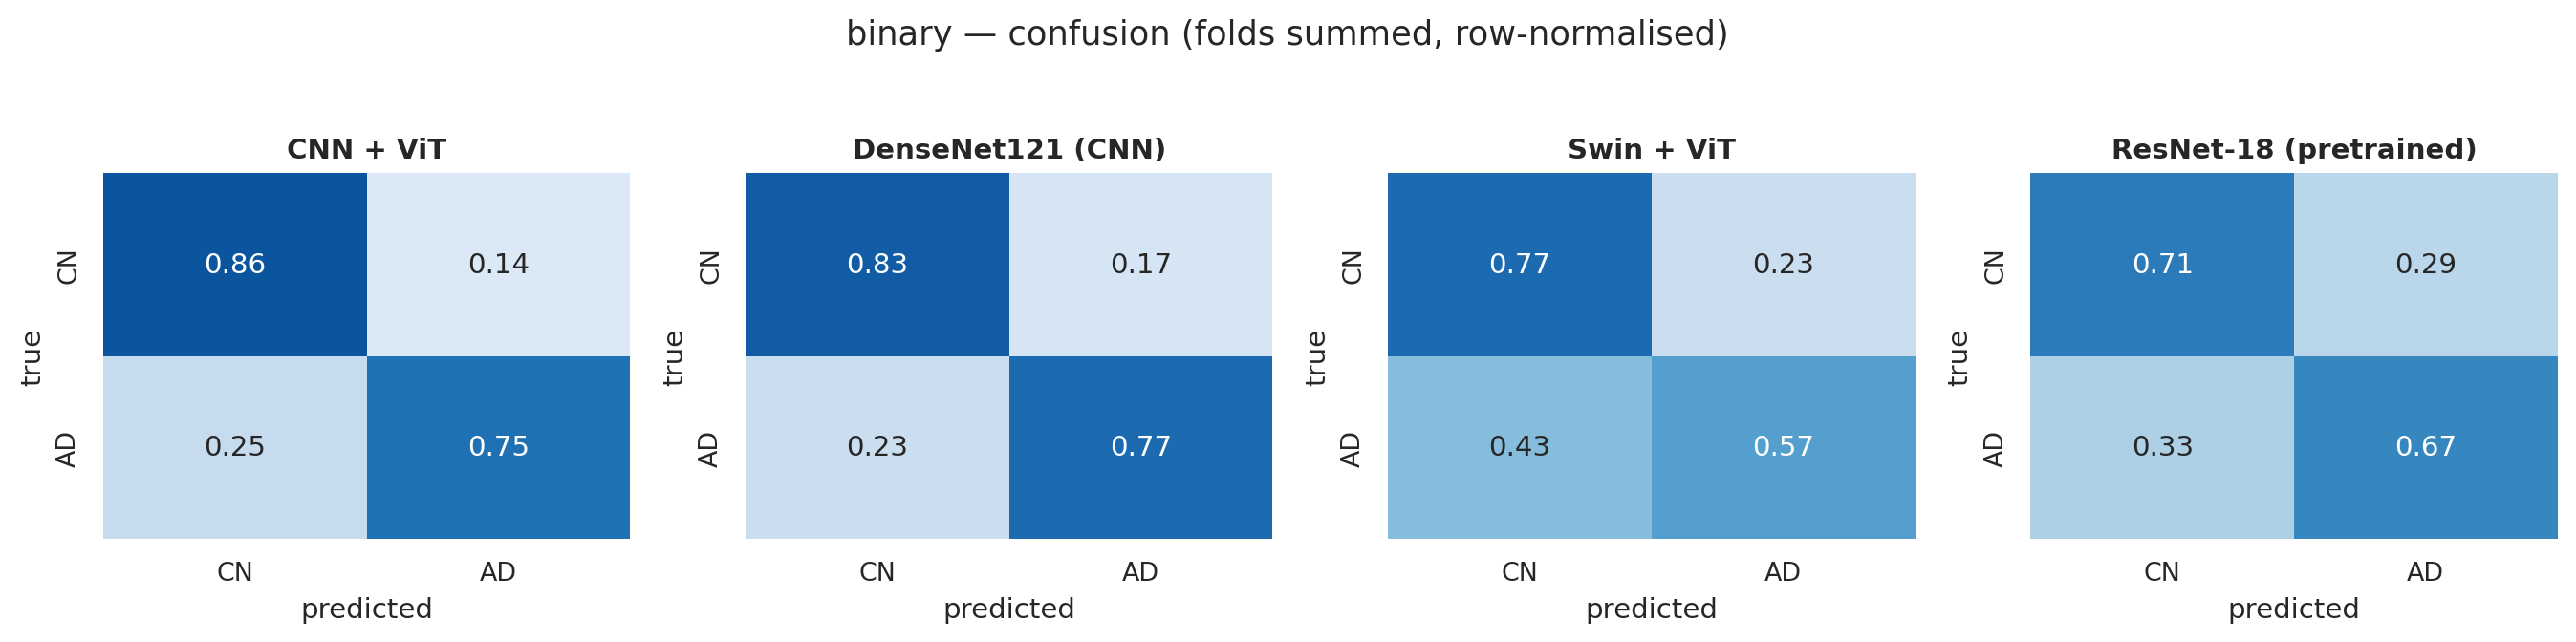
\includegraphics[width=10cm]{Images/res_confusion_binary.png}
    \caption[Binary confusion matrices]{\textbf{Binary confusion matrices.} Fold-summed, row-normalised CN-vs-AD confusion for all four binary models (subject-level predictions).}
    \label{fig:confusion_binary}
\end{figure}

\begin{figure}[H]
    \centering
    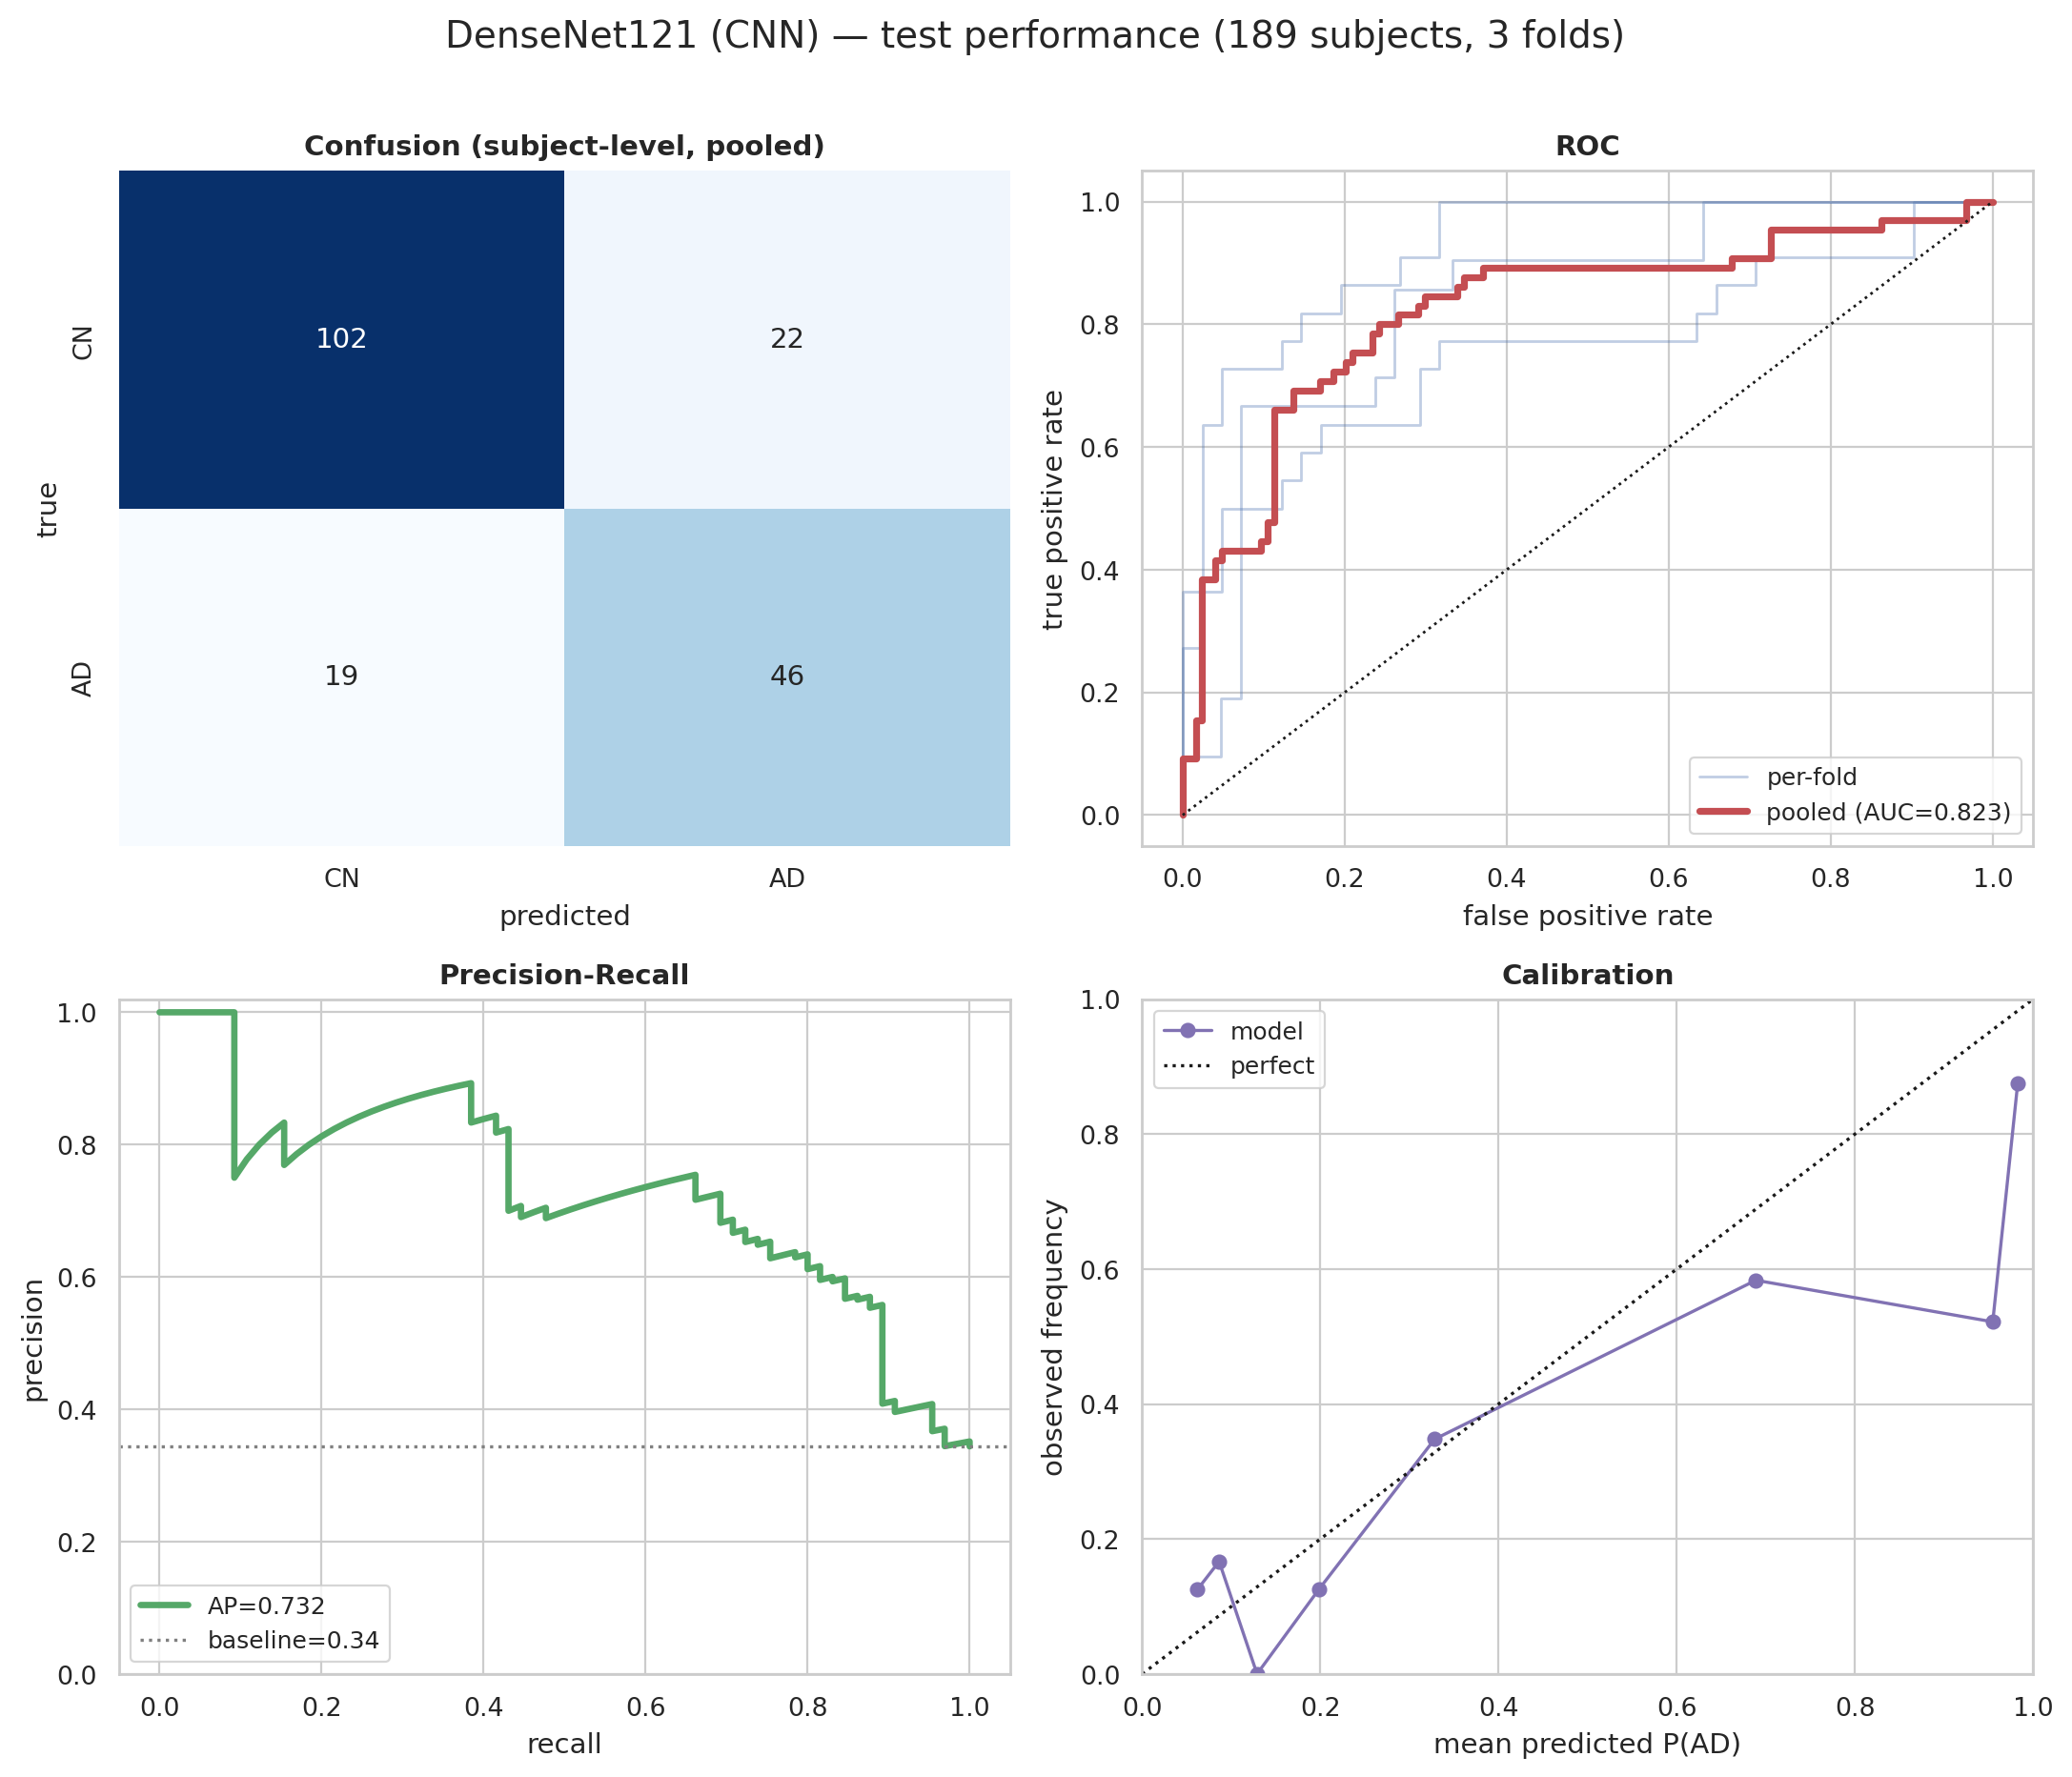
\includegraphics[width=15cm]{Images/res_perf_binary_cnn.png}
    \caption[Binary diagnostics (3 of 5 folds)]{\textbf{Binary diagnostics (3 of 5 folds, 189 subjects).} Confusion, per-fold and pooled ROC, precision--recall, and calibration for the 3D CNN (CN-vs-AD), computed on the three folds whose checkpoints were retained.}
    \label{fig:perf_binary}
\end{figure}

\section{Three-Class CN/MCI/AD Results (Honest Benchmark)}
Adding MCI --- the transitional stage whose MRI signature overlaps both neighbours --- sharply lowers performance for every model (Table~\ref{tab:3class}). The Swin Transformer and the 3D CNN are tied at the top ($\sim\!57\%$ accuracy, $\sim\!0.53$ macro-F1; paired fold-wise test $t=0.70$, $p\approx0.5$), only about five points above the $52.2\%$ accuracy of always predicting CN --- although their macro-F1 is more than twice the baseline's $0.23$, showing that they do separate the classes to some degree. The from-scratch ViT falls \emph{below} the majority baseline (Section~\ref{sec:vit_collapse}). The proposed CNN--ViT hybrid was not trained on the three-class task.

\begin{table}[H]
\centering
\caption{Three-class CN/MCI/AD, subject-level 5-fold cross-validation (mean $\pm$ std).}
\label{tab:3class}
\begin{tabular}{|l|c|c|c|}
\hline
\textbf{Model} & \textbf{Accuracy} & \textbf{Macro-F1} & \textbf{Weighted-F1} \\
\hline
\textbf{Swin Transformer} & \textbf{0.577 $\pm$ 0.098} & \textbf{0.537 $\pm$ 0.078} & \textbf{0.573} \\
3D CNN (DenseNet-121, scratch) & 0.572 $\pm$ 0.092 & 0.524 $\pm$ 0.071 & 0.560 \\
3D ViT (from scratch) & 0.286 $\pm$ 0.015 & 0.256 $\pm$ 0.012 & 0.184 \\
\hline
\textit{Majority-class baseline (always CN)} & \textit{0.522} & \textit{0.229} & \textit{0.358} \\
\hline
\end{tabular}
\end{table}

\begin{figure}[H]
    \centering
    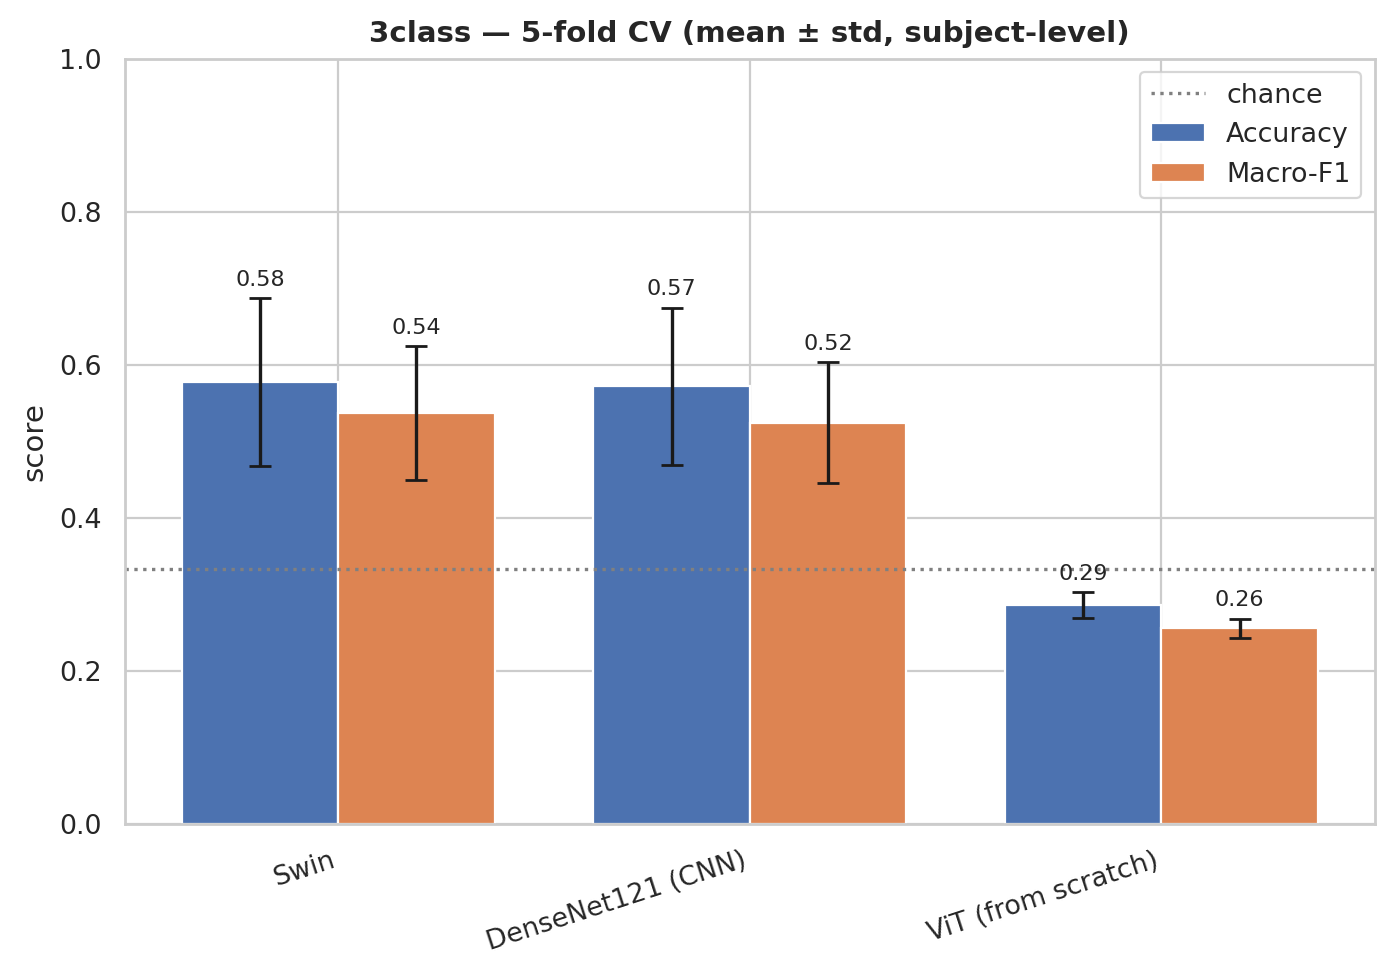
\includegraphics[width=14cm]{Images/res_bar_3class.png}
    \caption[Three-class model comparison]{\textbf{Three-class model comparison.} Per-model accuracy, macro-F1, and weighted-F1 for CN/MCI/AD (mean $\pm$ std over five folds).}
    \label{fig:bar_3class}
\end{figure}

The per-class breakdown is revealing: pooled over folds, CN reaches a per-class F1 of about $0.65$ and AD $0.55$--$0.61$, whereas \textbf{MCI reaches only $0.37$--$0.41$} (Table~\ref{tab:3class_perclass}). The confusion is overwhelmingly MCI being absorbed into CN or AD, exactly as expected for a stage that is clinically defined as intermediate. This is why a leakage-free three-class accuracy in the high-90s (as claimed by several slice-level studies in Chapter~\ref{cha:LiteratureReviewU}) is not credible on 395 subjects: the ceiling here is honest, and MCI is the bottleneck.

\section{Per-Fold Results and Fold Variance}
Because the cohort is small, a single split is unreliable; reporting every fold exposes how stable each model actually is. Tables~\ref{tab:binary_folds} and \ref{tab:3class_folds} give the per-fold macro-F1 for the binary and three-class tasks, and Figure~\ref{fig:box} shows the corresponding spread.

\begin{table}[H]
\centering
\caption{Binary CN-vs-AD per-fold macro-F1 (subject-level).}
\label{tab:binary_folds}
\begin{tabular}{|l|c|c|c|c|c|c|}
\hline
\textbf{Model} & \textbf{F1} & \textbf{F2} & \textbf{F3} & \textbf{F4} & \textbf{F5} & \textbf{Mean $\pm$ std} \\
\hline
Hybrid CNN--ViT & 0.716 & 0.857 & 0.743 & 0.821 & 0.873 & \textbf{0.802 $\pm$ 0.062} \\
CNN (DenseNet) & 0.768 & 0.810 & 0.678 & 0.834 & 0.850 & 0.788 $\pm$ 0.062 \\
Hybrid Swin--ViT & 0.672 & 0.723 & 0.700 & 0.750 & 0.466 & 0.662 $\pm$ 0.101 \\
ResNet (pretrained) & 0.775 & 0.449 & 0.449 & 0.779 & 0.816 & 0.654 $\pm$ 0.168 \\
\hline
\end{tabular}
\end{table}

The ResNet row is the clearest illustration of instability: three folds are strong ($\sim\!0.78$--$0.82$) while two collapse to $0.449$, halving the mean and inflating the standard deviation. This bimodal pattern --- rather than a uniformly weak model --- is consistent with the early-stopping hypothesis discussed below. By contrast, the CNN and the CNN--ViT hybrid stay above $0.67$ macro-F1 in every fold, although each still varies by about $0.15$--$0.17$ between its best and worst fold.

\begin{table}[H]
\centering
\caption{Three-class CN/MCI/AD per-fold macro-F1 (subject-level).}
\label{tab:3class_folds}
\begin{tabular}{|l|c|c|c|c|c|c|}
\hline
\textbf{Model} & \textbf{F1} & \textbf{F2} & \textbf{F3} & \textbf{F4} & \textbf{F5} & \textbf{Mean $\pm$ std} \\
\hline
Swin Transformer & 0.564 & 0.471 & 0.457 & 0.675 & 0.518 & \textbf{0.537 $\pm$ 0.078} \\
CNN (DenseNet) & 0.592 & 0.433 & 0.489 & 0.622 & 0.487 & 0.524 $\pm$ 0.071 \\
ViT (scratch) & 0.261 & 0.238 & 0.254 & 0.273 & 0.253 & 0.256 $\pm$ 0.012 \\
\hline
\end{tabular}
\end{table}

\begin{figure}[H]
    \centering
    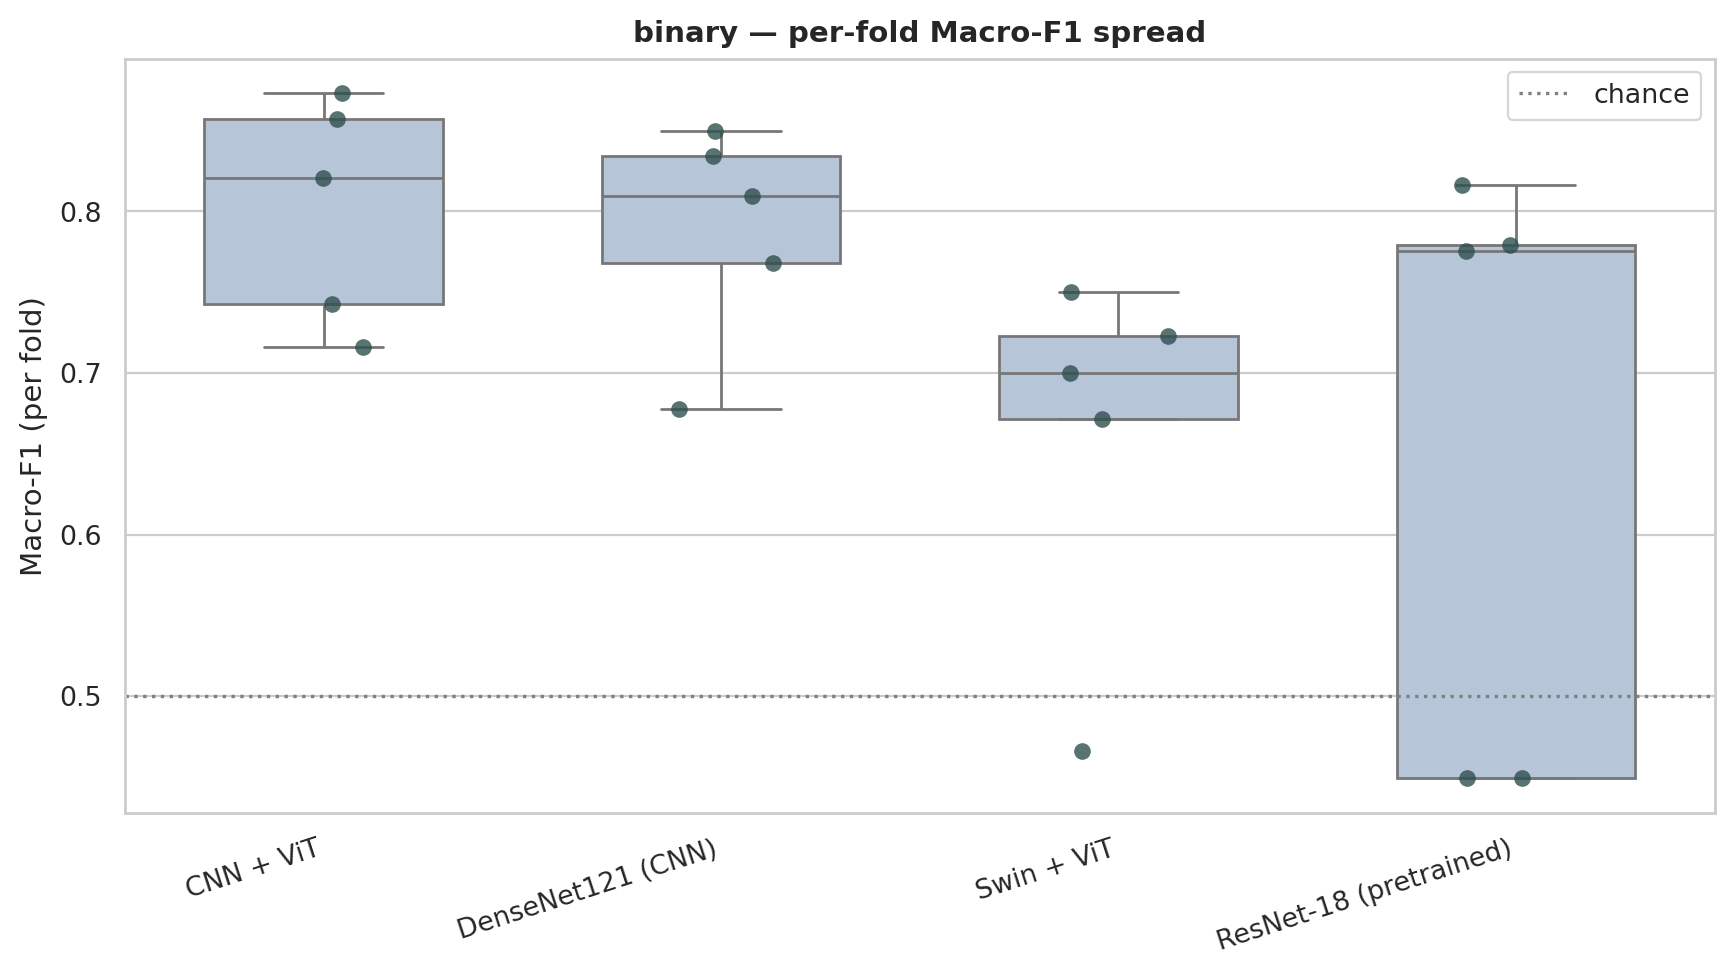
\includegraphics[width=7.6cm]{Images/res_box_binary.png}\hfill
    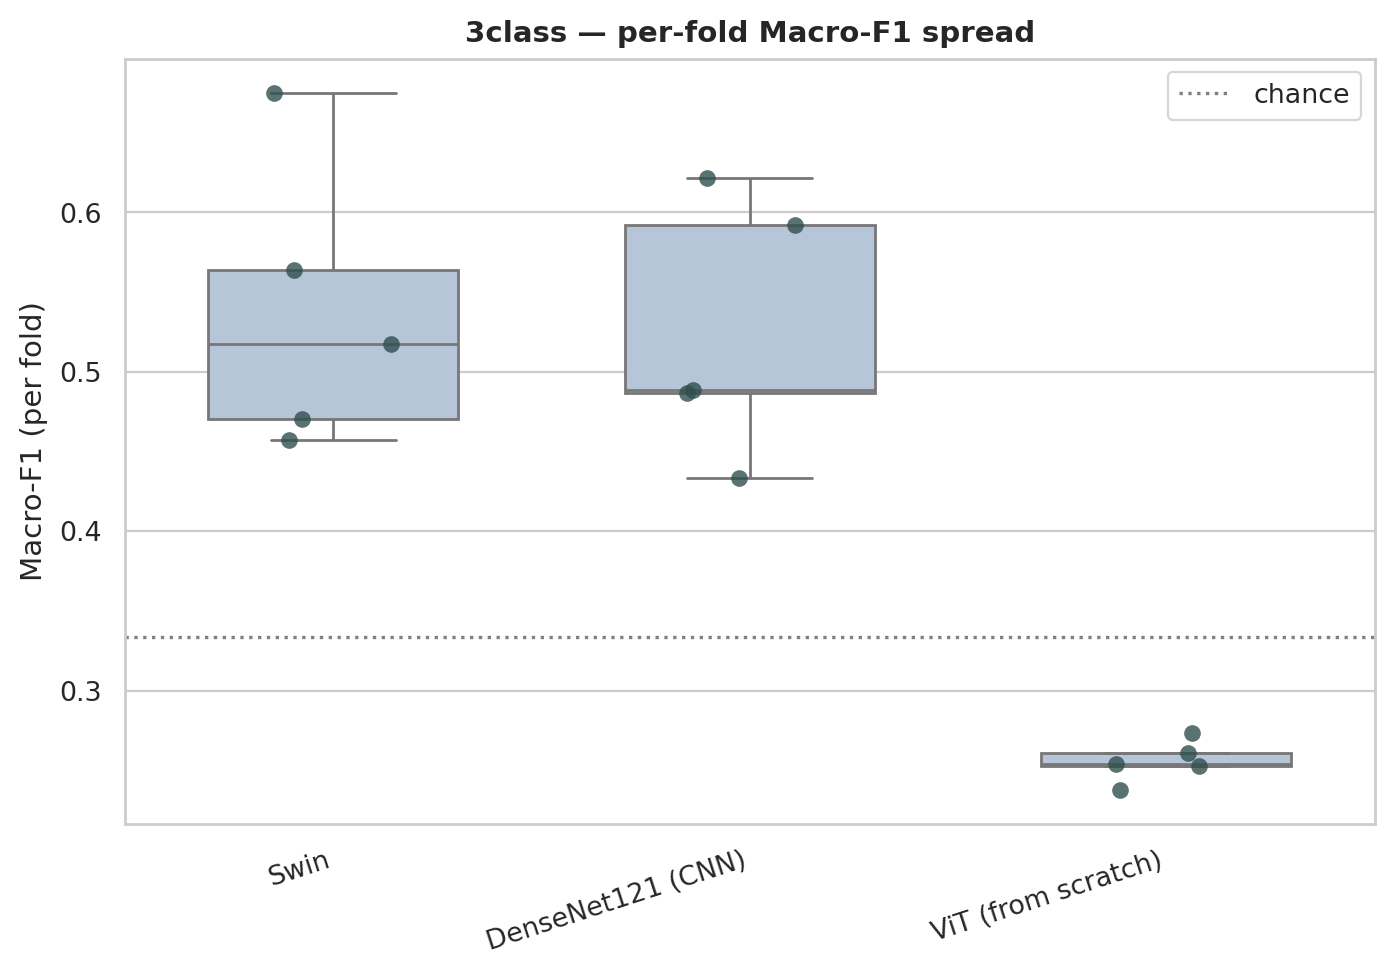
\includegraphics[width=7.6cm]{Images/res_box_3class.png}
    \caption[Fold variance]{\textbf{Fold variance.} Per-fold spread of macro-F1 for the binary (left) and three-class (right) tasks.}
    \label{fig:box}
\end{figure}

\section{Per-Class Performance}
Tables~\ref{tab:binary_perclass} and \ref{tab:3class_perclass} give the pooled per-class precision, recall, and F1 (aggregated over all five test folds). In the binary task both classes are recovered well, with the smaller AD class trailing the majority CN class by roughly $0.11$--$0.12$ F1 --- a modest, expected imbalance gap. In the three-class task the picture is dominated by MCI: its F1 ($0.37$--$0.41$) is only about half that of CN, and its low recall shows that a large fraction of true MCI subjects are pushed into the neighbouring CN or AD classes. This quantifies the qualitative claim that MCI is the bottleneck of the whole problem.

\begin{table}[H]
\centering
\caption{Binary CN-vs-AD pooled per-class metrics.}
\label{tab:binary_perclass}
\begin{tabular}{|l|l|c|c|c|c|}
\hline
\textbf{Model} & \textbf{Class} & \textbf{Precision} & \textbf{Recall} & \textbf{F1} & \textbf{Support} \\
\hline
\multirow{2}{*}{Hybrid CNN--ViT} & CN & 0.868 & 0.859 & 0.863 & 206 \\
                                 & AD & 0.739 & 0.752 & 0.745 & 109 \\
\hline
\multirow{2}{*}{CNN (DenseNet)}  & CN & 0.872 & 0.830 & 0.851 & 206 \\
                                 & AD & 0.706 & 0.771 & 0.737 & 109 \\
\hline
\end{tabular}
\end{table}

\begin{table}[H]
\centering
\caption{Three-class CN/MCI/AD pooled per-class metrics.}
\label{tab:3class_perclass}
\begin{tabular}{|l|l|c|c|c|c|}
\hline
\textbf{Model} & \textbf{Class} & \textbf{Precision} & \textbf{Recall} & \textbf{F1} & \textbf{Support} \\
\hline
\multirow{3}{*}{Swin} & CN  & 0.685 & 0.612 & 0.646 & 206 \\
                      & MCI & 0.366 & 0.375 & 0.370 & 80 \\
                      & AD  & 0.558 & 0.661 & 0.605 & 109 \\
\hline
\multirow{3}{*}{CNN}  & CN  & 0.653 & 0.641 & 0.647 & 206 \\
                      & MCI & 0.416 & 0.400 & 0.408 & 80 \\
                      & AD  & 0.534 & 0.569 & 0.551 & 109 \\
\hline
\end{tabular}
\end{table}

\section{Training Dynamics}
Figure~\ref{fig:tc} plots the training loss and validation subject-level macro-F1 across epochs for two representative binary runs. The from-scratch CNN's training loss falls steadily, while its validation macro-F1 rises to the $0.75$--$0.9$ range but fluctuates by up to $\pm0.1$ from epoch to epoch (only the folds whose logs were retained are plotted). The transformer-heavy runs are noisier and slower to rise, consistent with their weaker inductive bias. Figure~\ref{fig:tc_vit} shows the three-class ViT: its training loss barely decreases and its validation macro-F1 stays between about $0.1$ and $0.25$ throughout, a training-curve view of its collapse.

\begin{figure}[H]
    \centering
    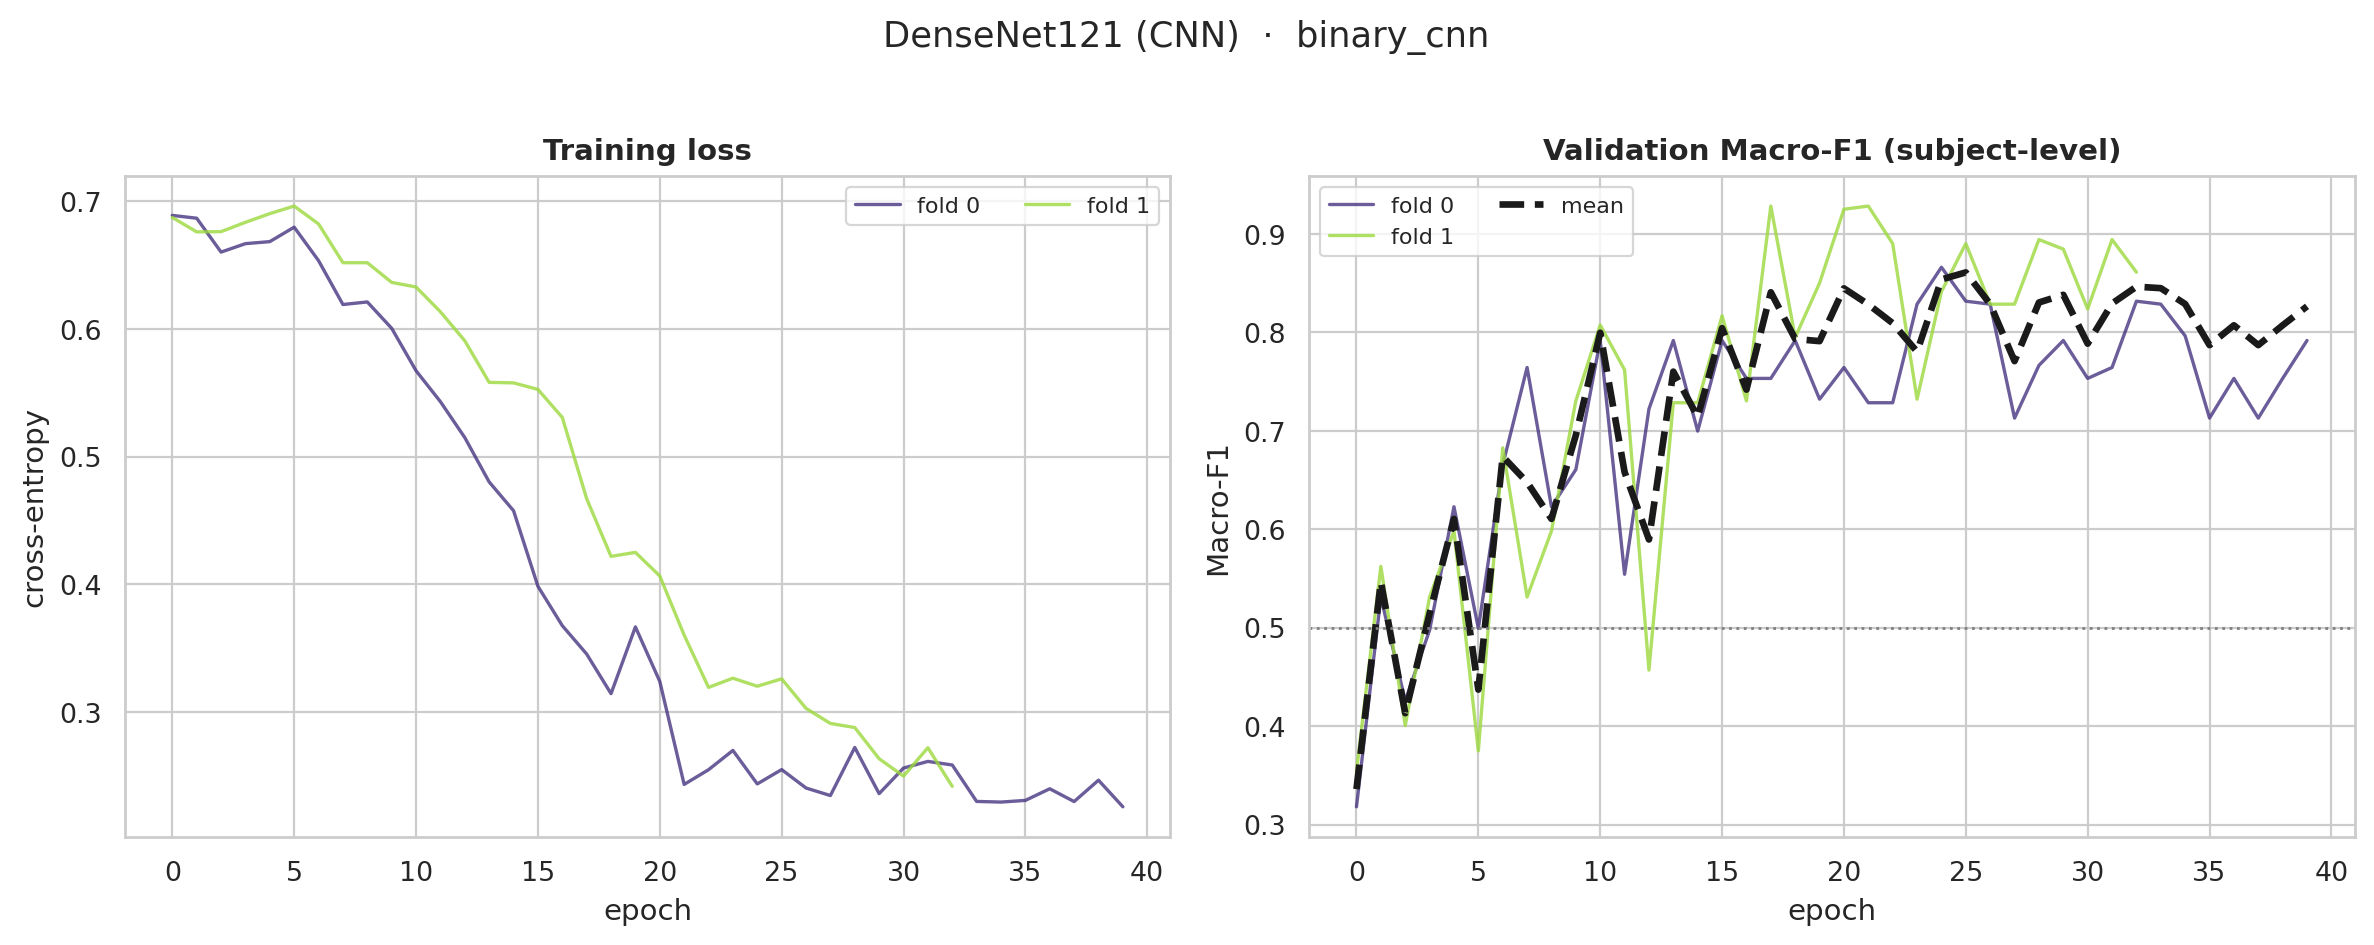
\includegraphics[width=7.6cm]{Images/tc_binary_cnn.png}\hfill
    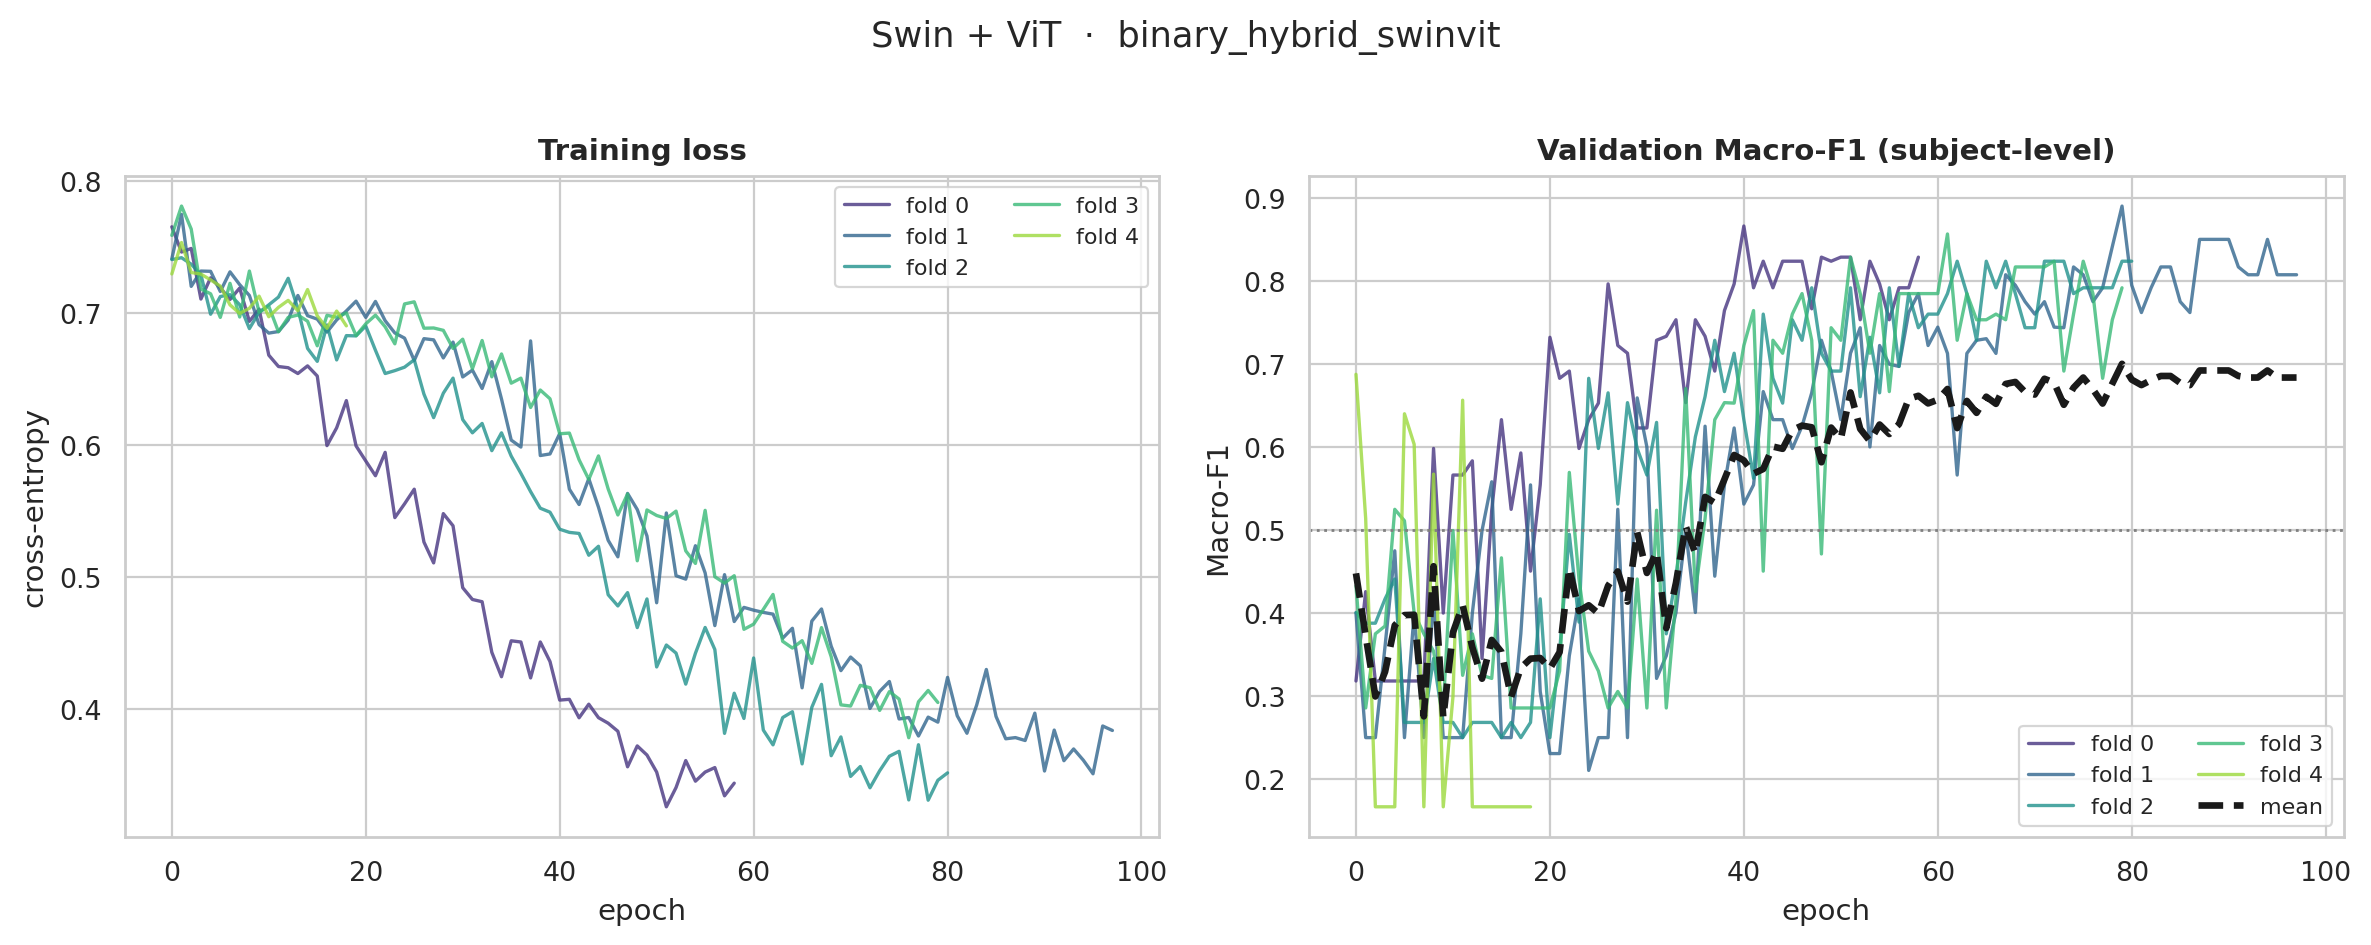
\includegraphics[width=7.6cm]{Images/tc_binary_hybrid_swinvit.png}
    \caption[Binary training curves]{\textbf{Binary training curves.} Per-fold training loss and validation macro-F1: binary CNN (left) and binary Swin--ViT hybrid (right).}
    \label{fig:tc}
\end{figure}

\begin{figure}[H]
    \centering
    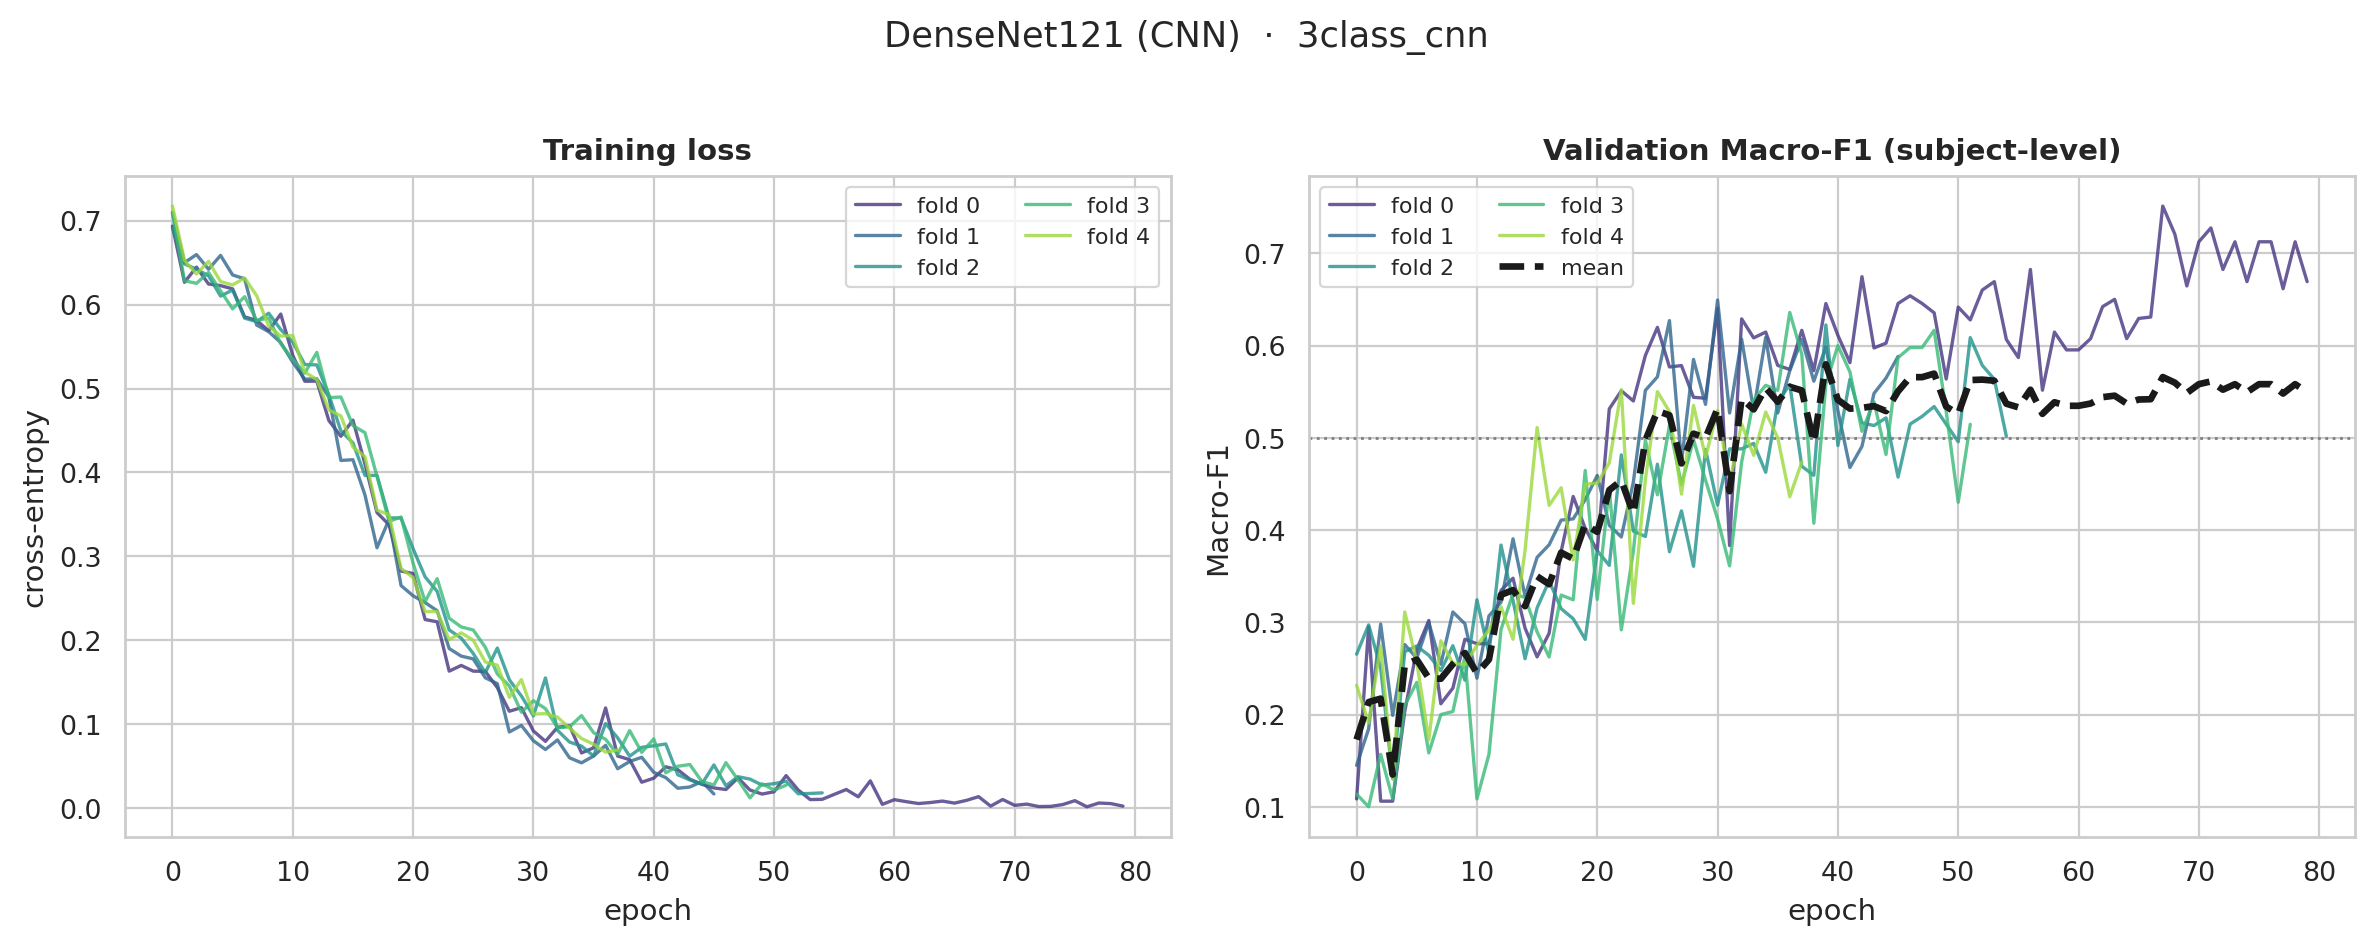
\includegraphics[width=7.6cm]{Images/tc_3class_cnn.png}\hfill
    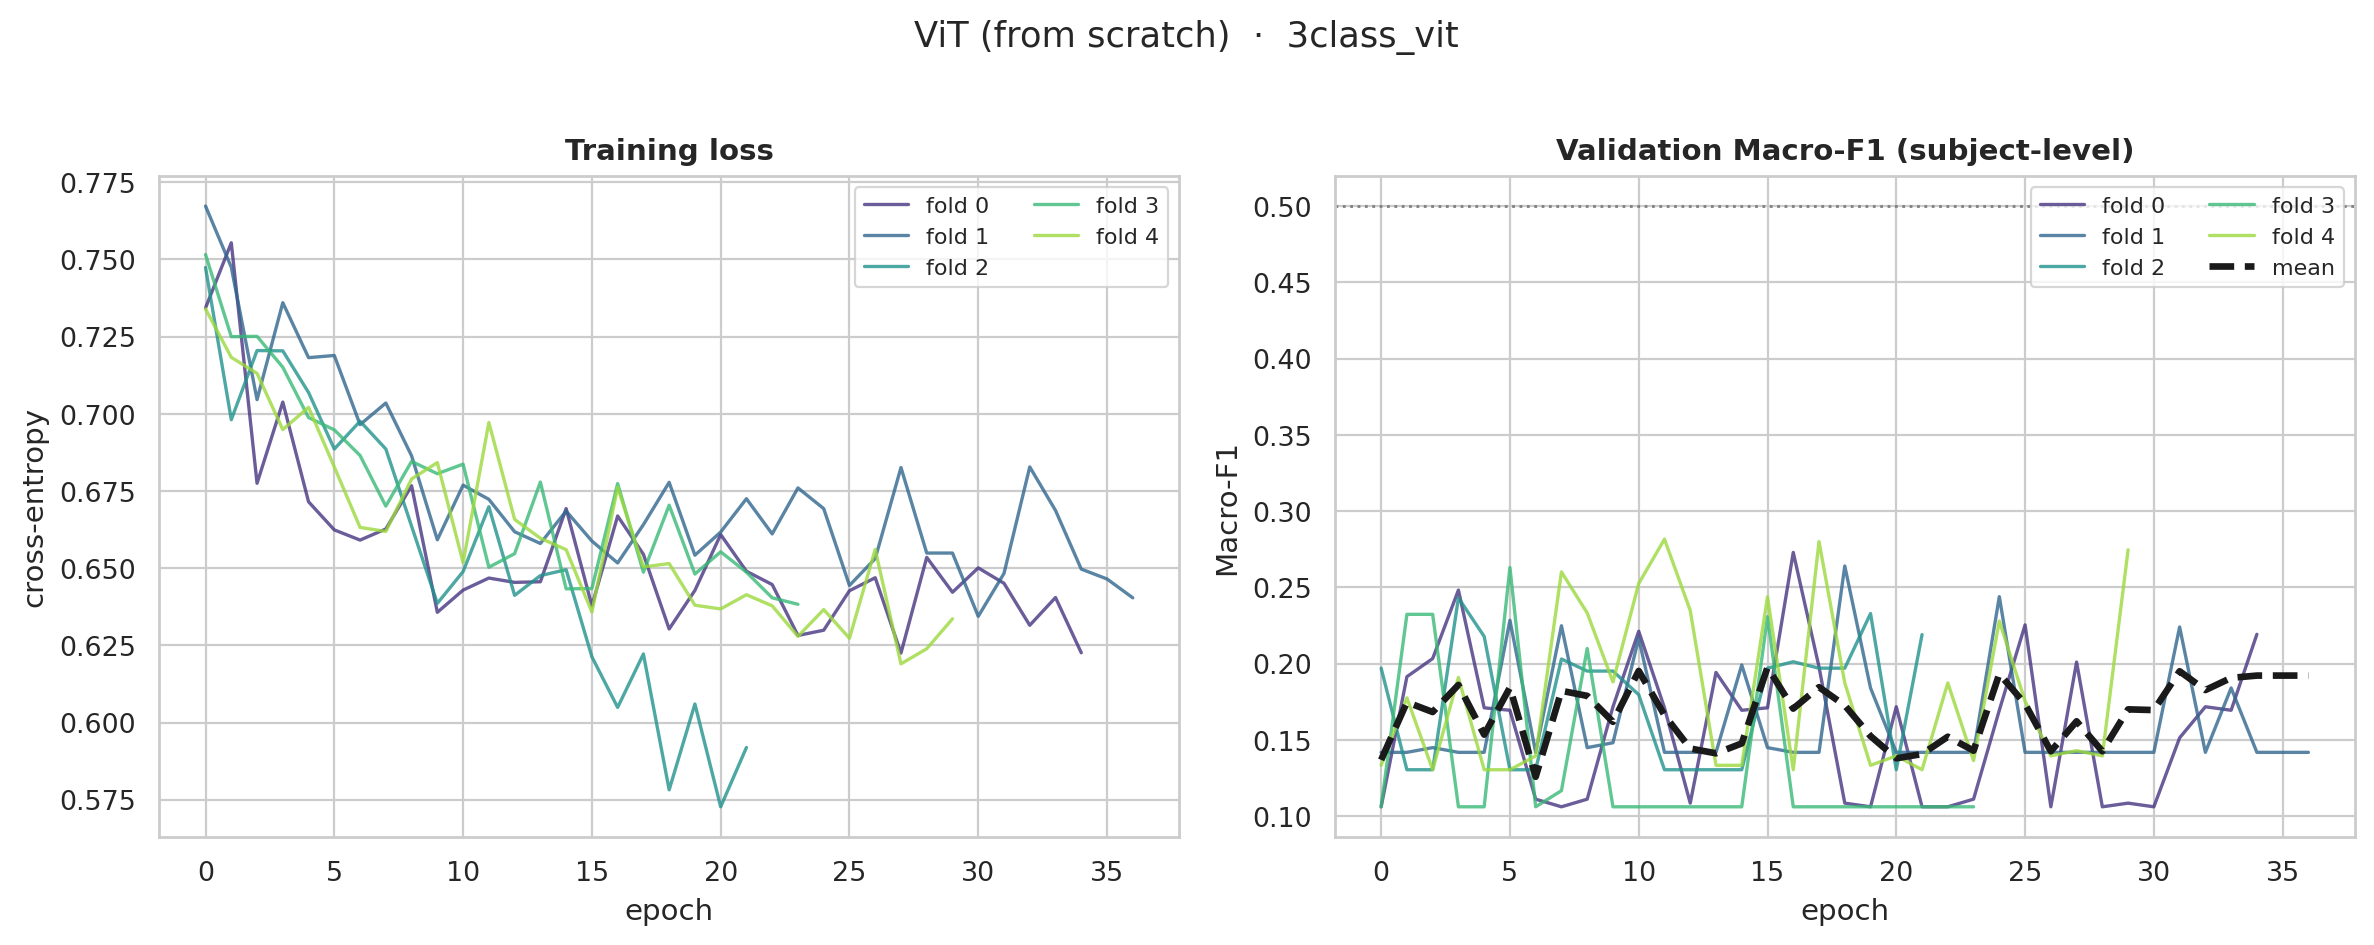
\includegraphics[width=7.6cm]{Images/tc_3class_vit.png}
    \caption[Three-class training dynamics]{\textbf{Three-class training dynamics.} DenseNet CNN (left) vs.\ from-scratch ViT (right; validation macro-F1 stays flat between about 0.1 and 0.25).}
    \label{fig:tc_vit}
\end{figure}

\section{Performance Diagnostics}
Beyond point metrics, Figure~\ref{fig:perf_extra} reports ROC, precision--recall, and calibration for the binary Swin--ViT hybrid and for the three-class CNN (one-vs-rest). The three-class one-vs-rest ROC gives AUCs of $0.69$ (CN), $0.66$ (MCI), and $0.77$ (AD): AD is the most separable class, MCI the least, and none is separated strongly --- echoing the confusion-matrix analysis.

\begin{figure}[H]
    \centering
    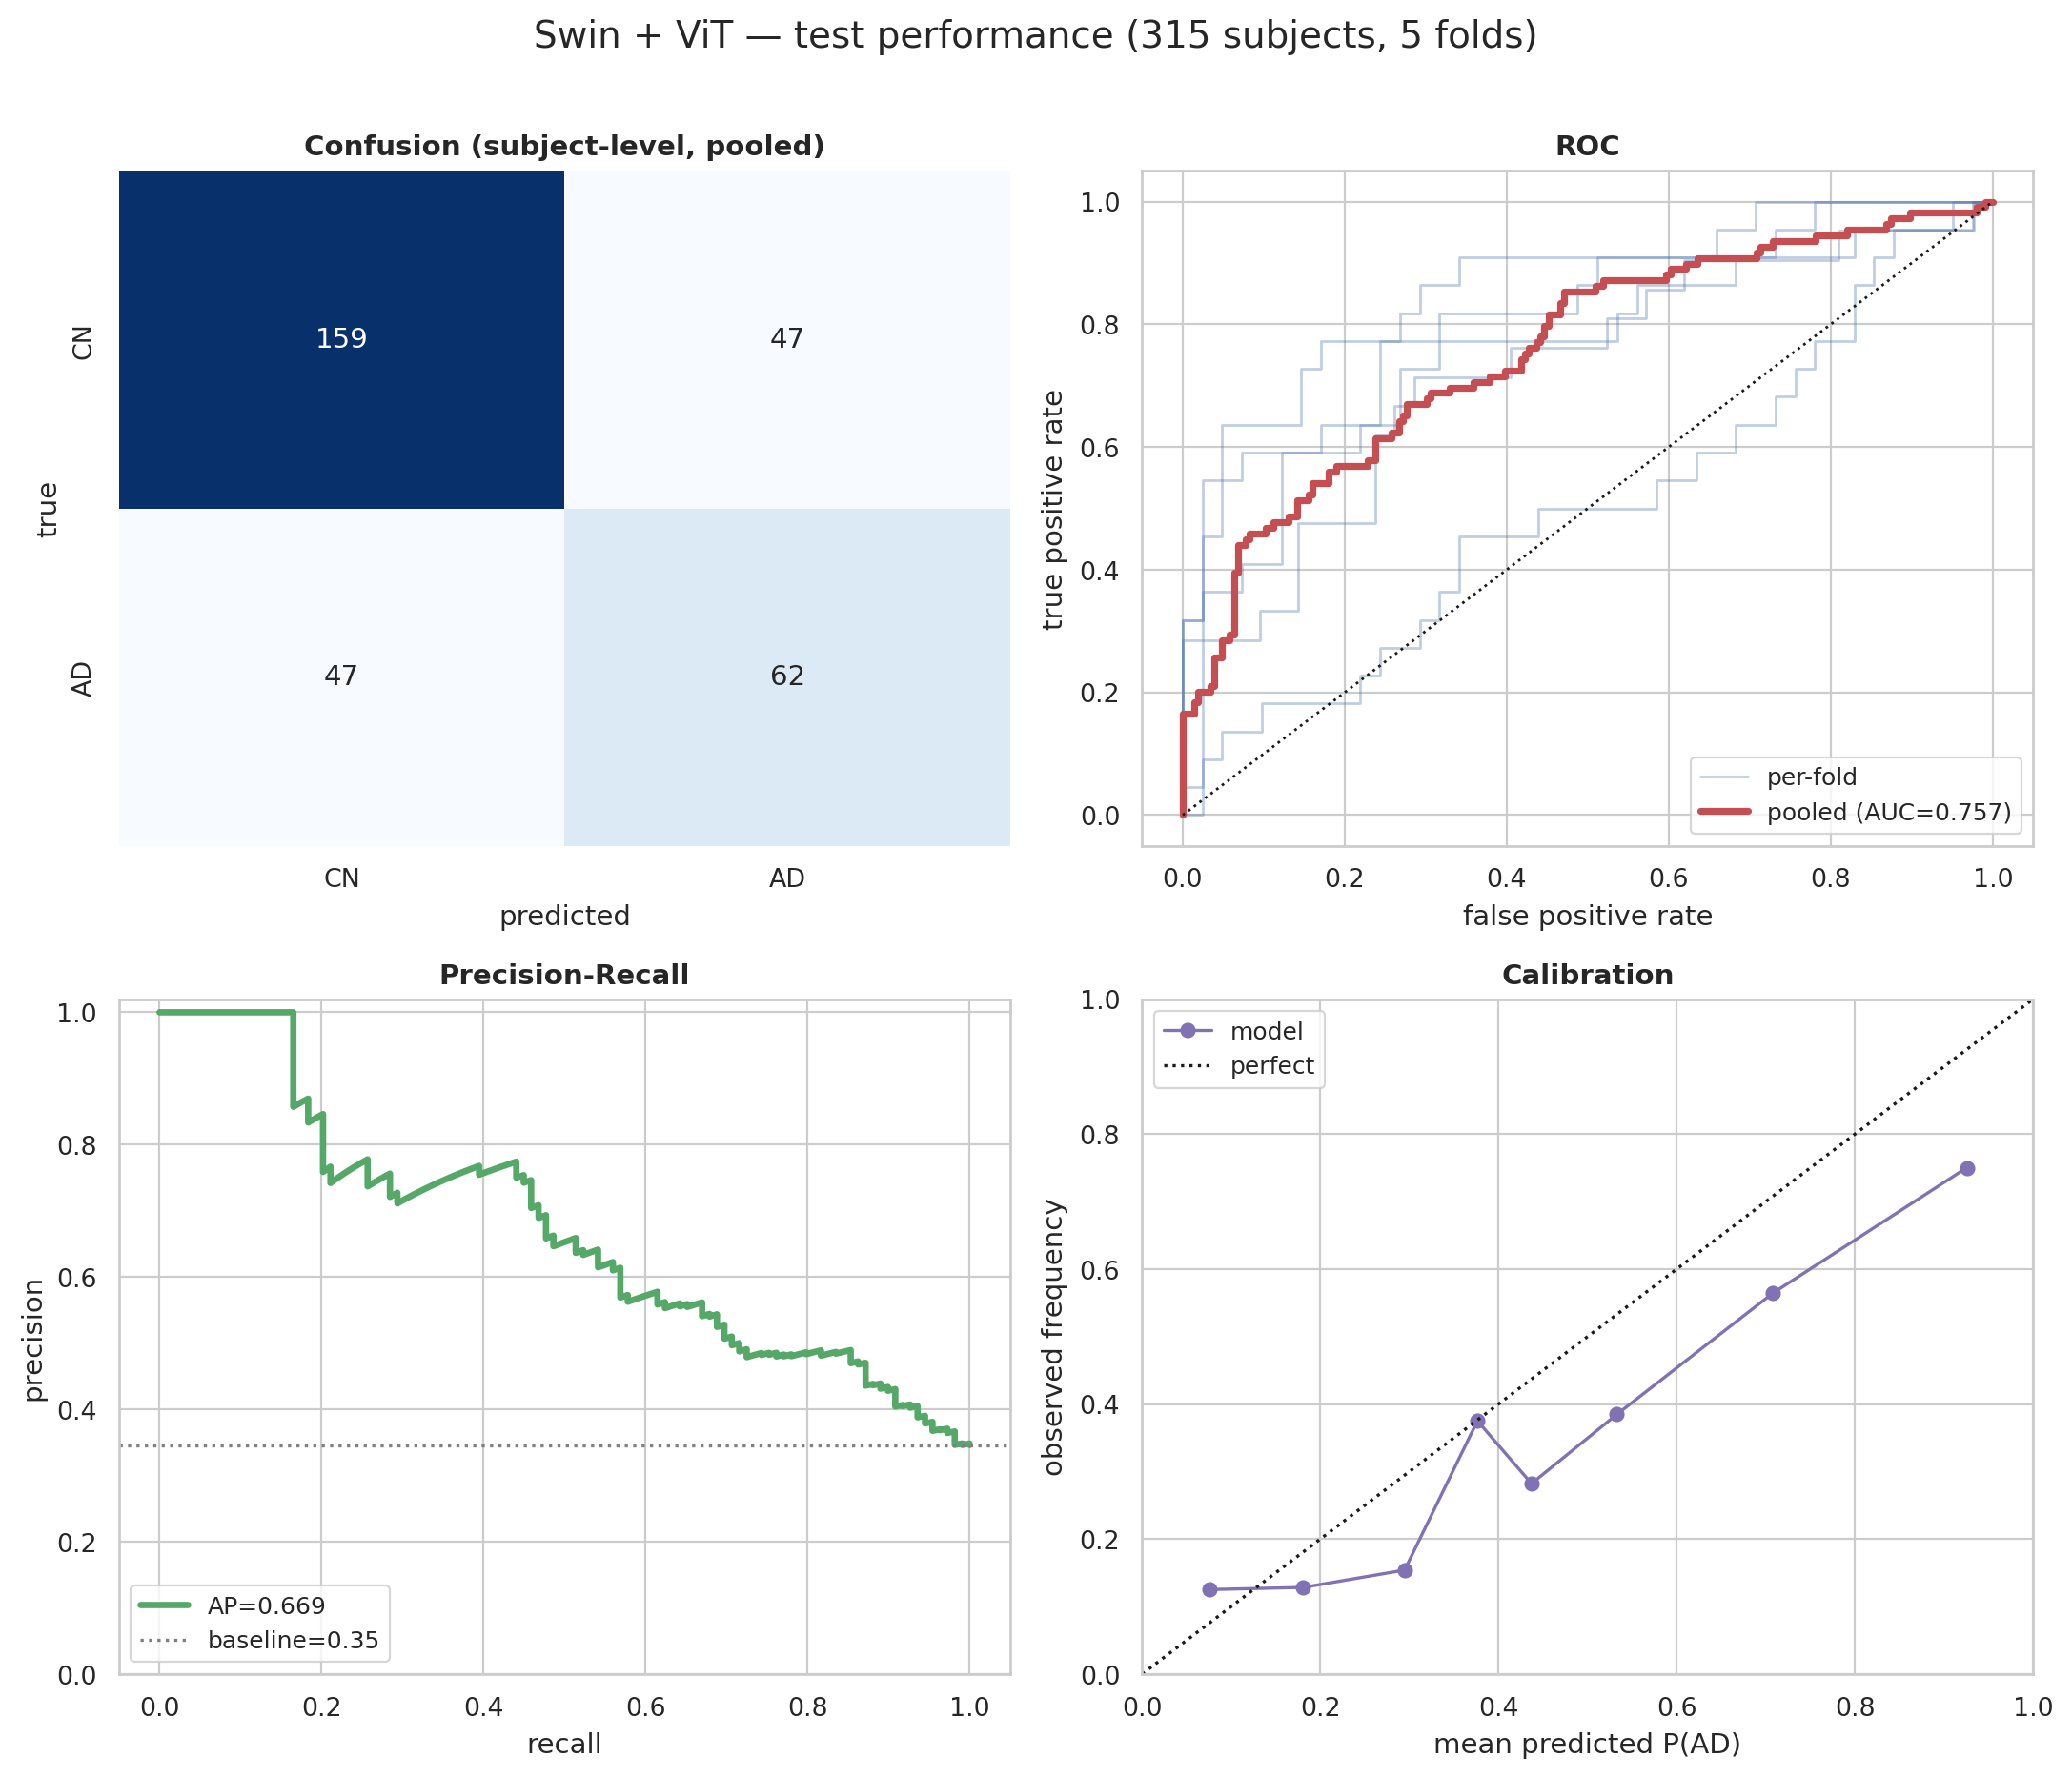
\includegraphics[width=7.6cm]{Images/perf_binary_hybrid_swinvit.png}\hfill
    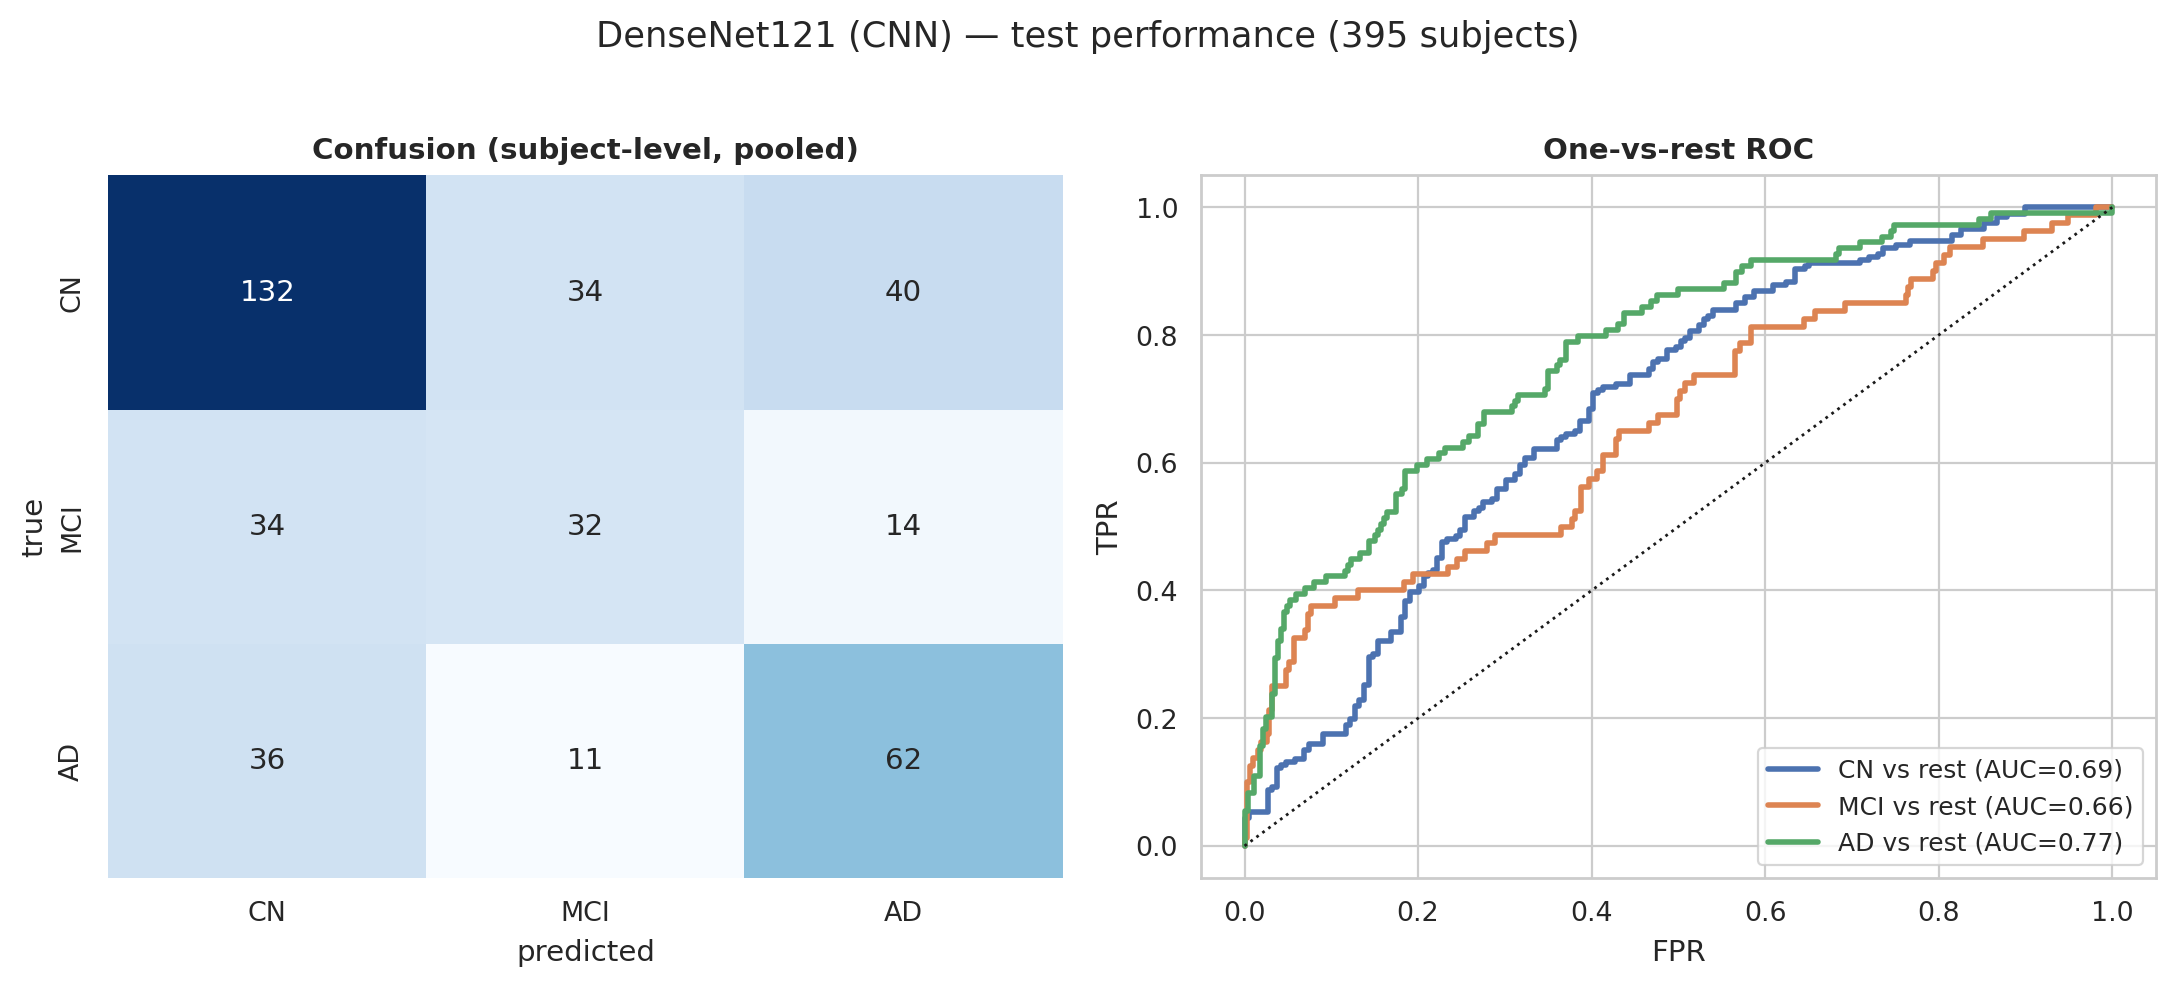
\includegraphics[width=7.6cm]{Images/perf_3class_cnn.png}
    \caption[Extended diagnostics]{\textbf{Extended diagnostics.} Binary Swin--ViT hybrid (left) and three-class CNN one-vs-rest (right).}
    \label{fig:perf_extra}
\end{figure}

\section{Feature-Space Analysis}
To see \emph{why} the models succeed or fail, Figure~\ref{fig:emb} projects the penultimate-layer features (one fold) with t-SNE. The binary CNN forms two largely separated CN/AD clusters, with the misclassified subjects concentrated in the region where they meet. For the three classes, the Swin encoder produces partially separable CN and AD regions with MCI scattered between them, whereas the from-scratch ViT produces a single undifferentiated blob --- a geometric picture of a model that never learned a useful representation.

\begin{figure}[H]
    \centering
    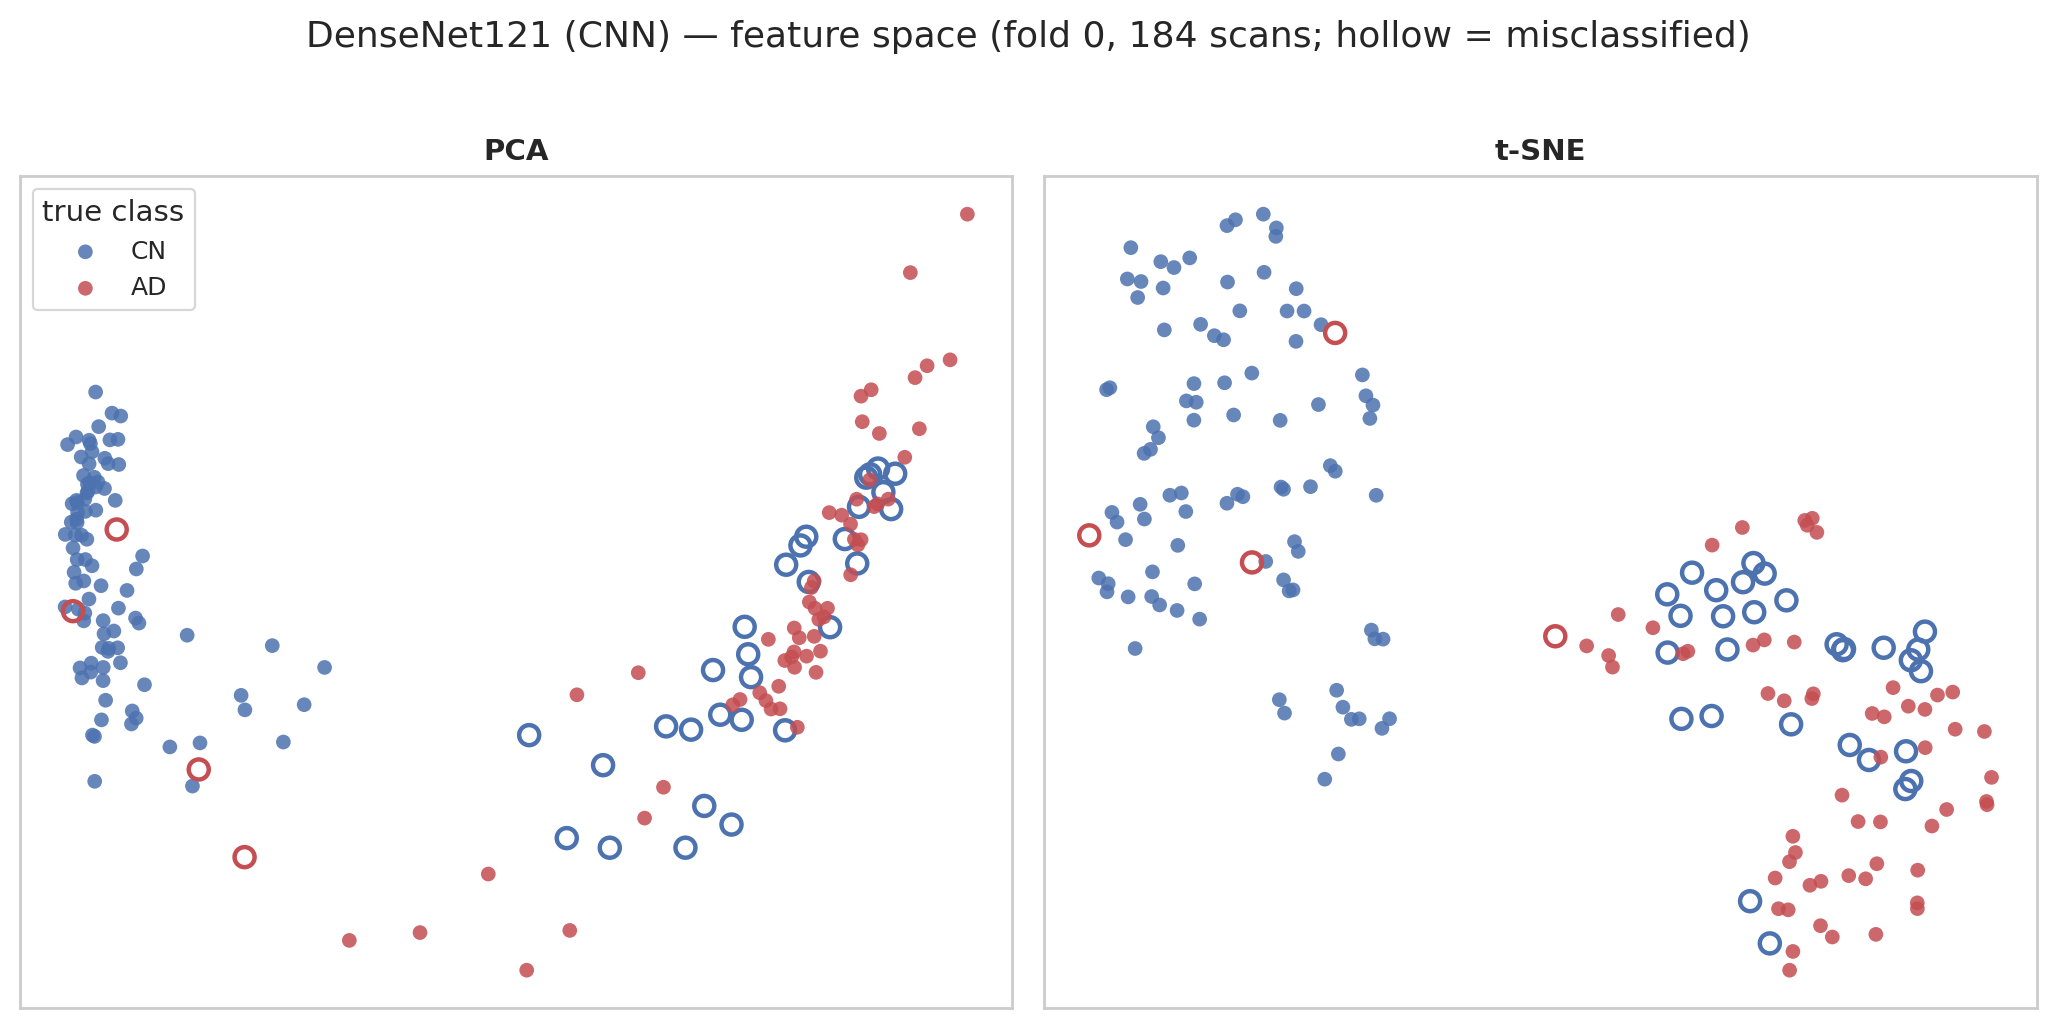
\includegraphics[width=5.1cm]{Images/emb_binary_cnn.png}\hfill
    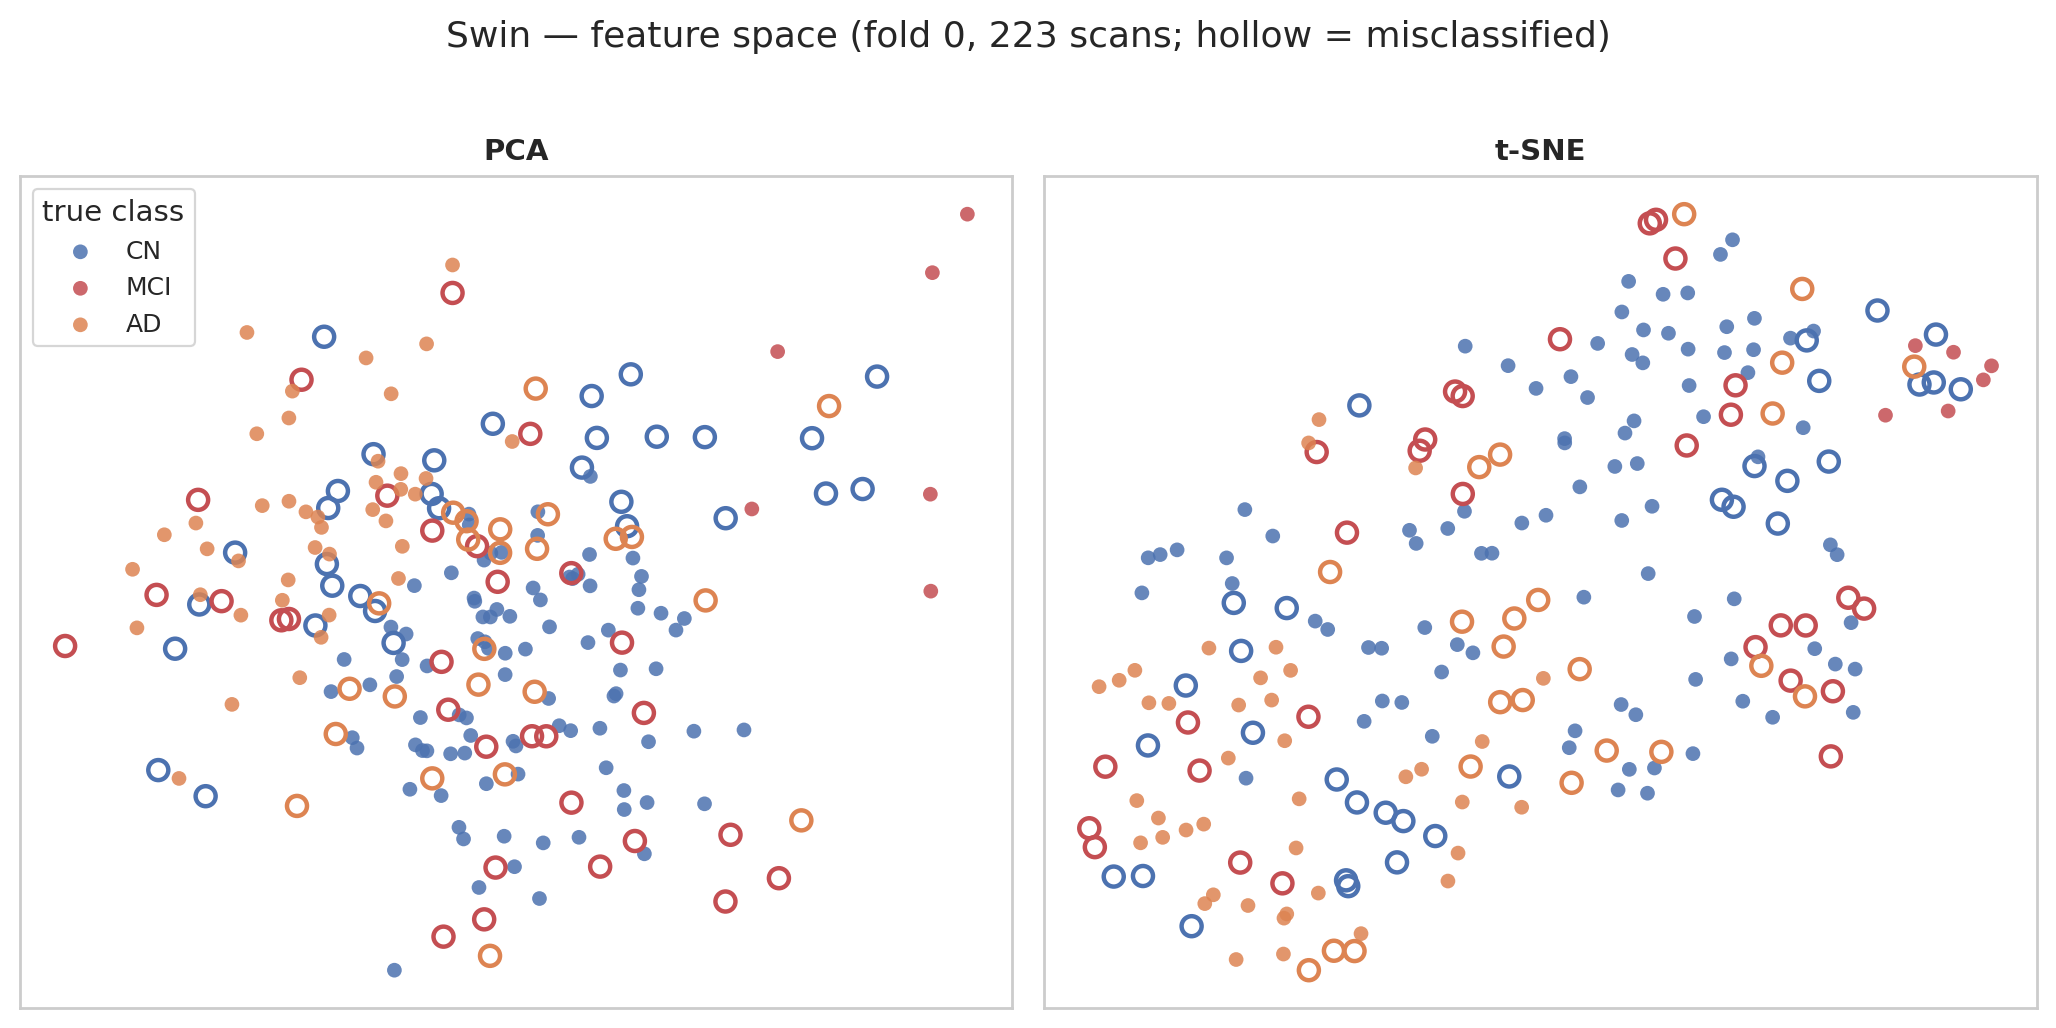
\includegraphics[width=5.1cm]{Images/emb_3class_swin.png}\hfill
    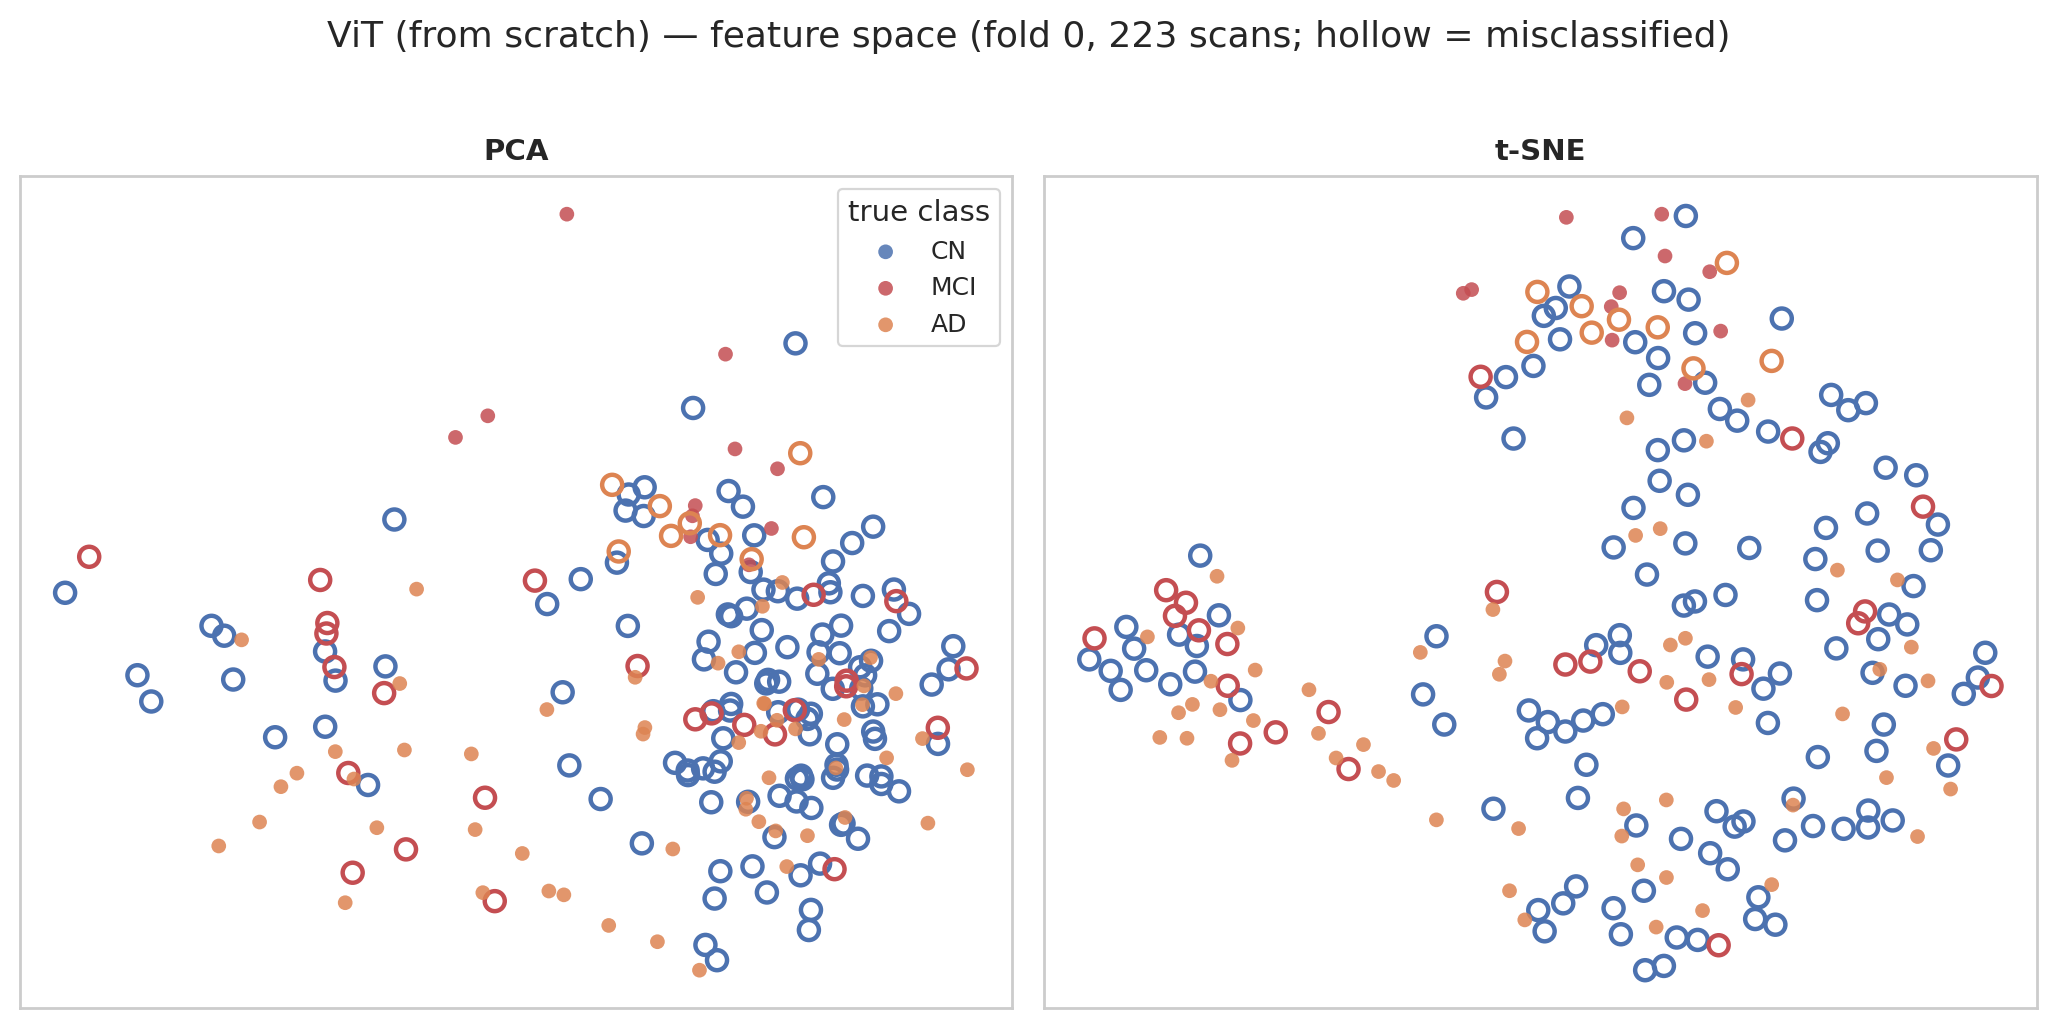
\includegraphics[width=5.1cm]{Images/emb_3class_vit.png}
    \caption[Feature embeddings]{\textbf{Feature embeddings.} t-SNE of penultimate features: binary CNN (left, two clean clusters), three-class Swin (middle, MCI between CN/AD), three-class ViT (right, collapsed).}
    \label{fig:emb}
\end{figure}

\section{Error Analysis}
Figure~\ref{fig:err} inspects the mistakes. The predicted-probability histogram by true class (three of five folds, 189 subjects) shows that many binary errors are \emph{confident}: of the 22 misclassified CN subjects, about 14 receive $P(\text{AD})>0.9$, and about 7 AD subjects receive $P(\text{AD})<0.1$. The gallery shows the most confident of these misclassifications. Confident errors of this kind are not explained by a soft decision boundary; plausible causes, still to be investigated, include label noise (for example, CN subjects who later converted), age-related atrophy in older CN subjects, and site or scanner effects. In the three-class case the per-class metrics (Table~\ref{tab:3class_perclass}) and confusion matrices show that most errors are MCI subjects assigned to CN or AD, which is consistent with MCI's intermediate clinical definition.

\begin{figure}[H]
    \centering
    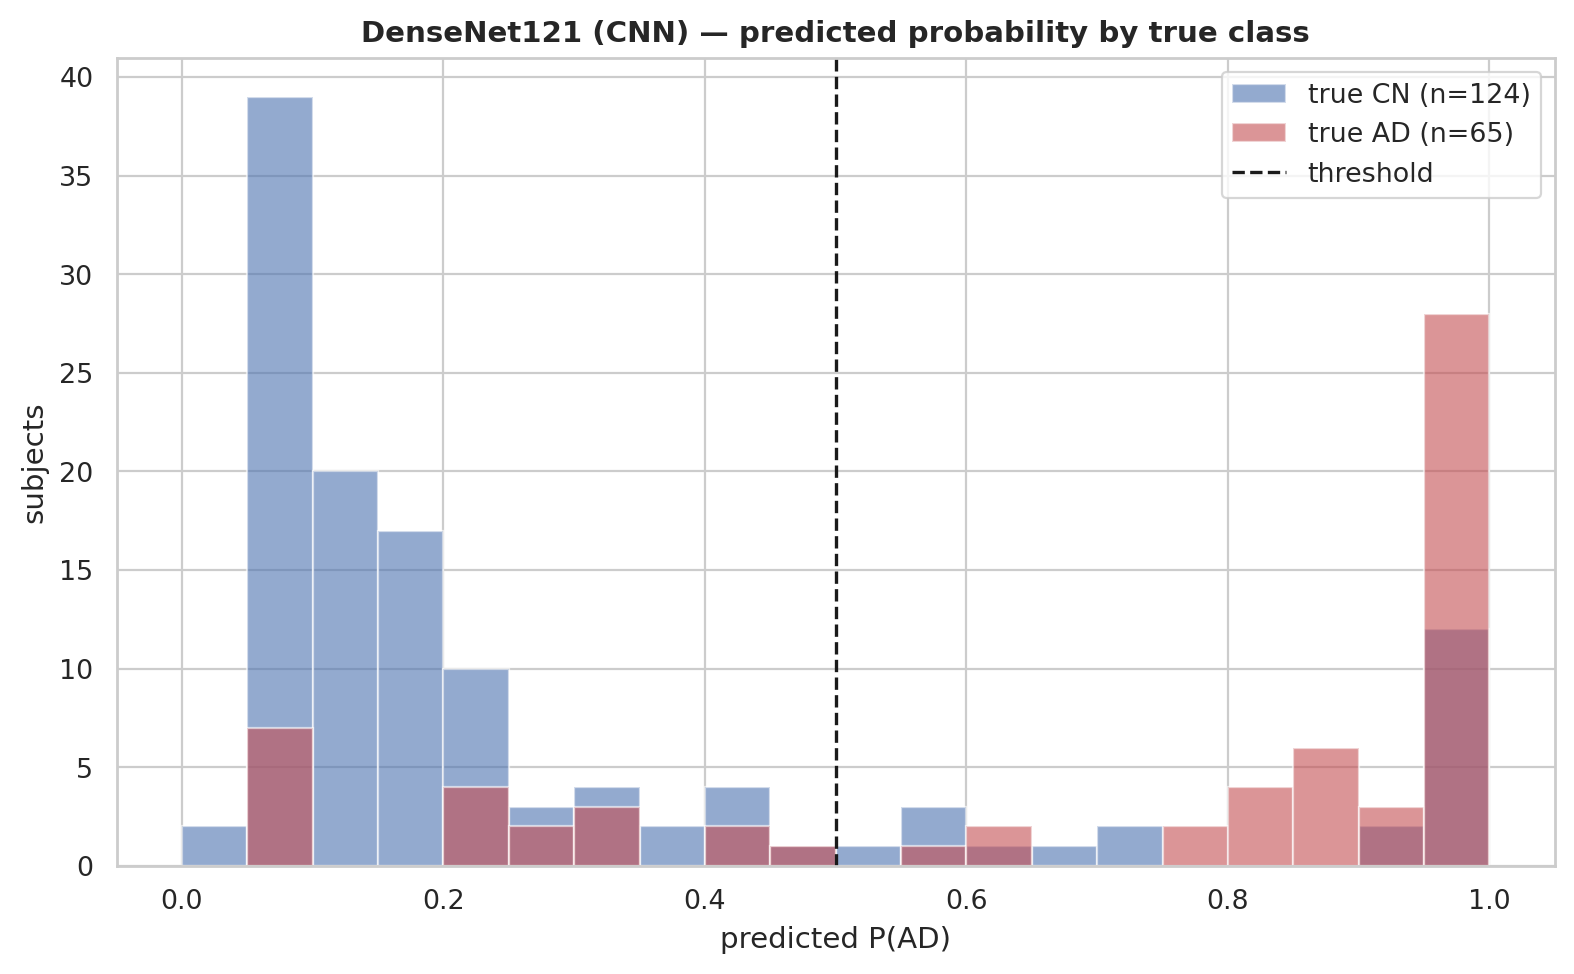
\includegraphics[width=7.6cm]{Images/err_binary_cnn_hist.png}\hfill
    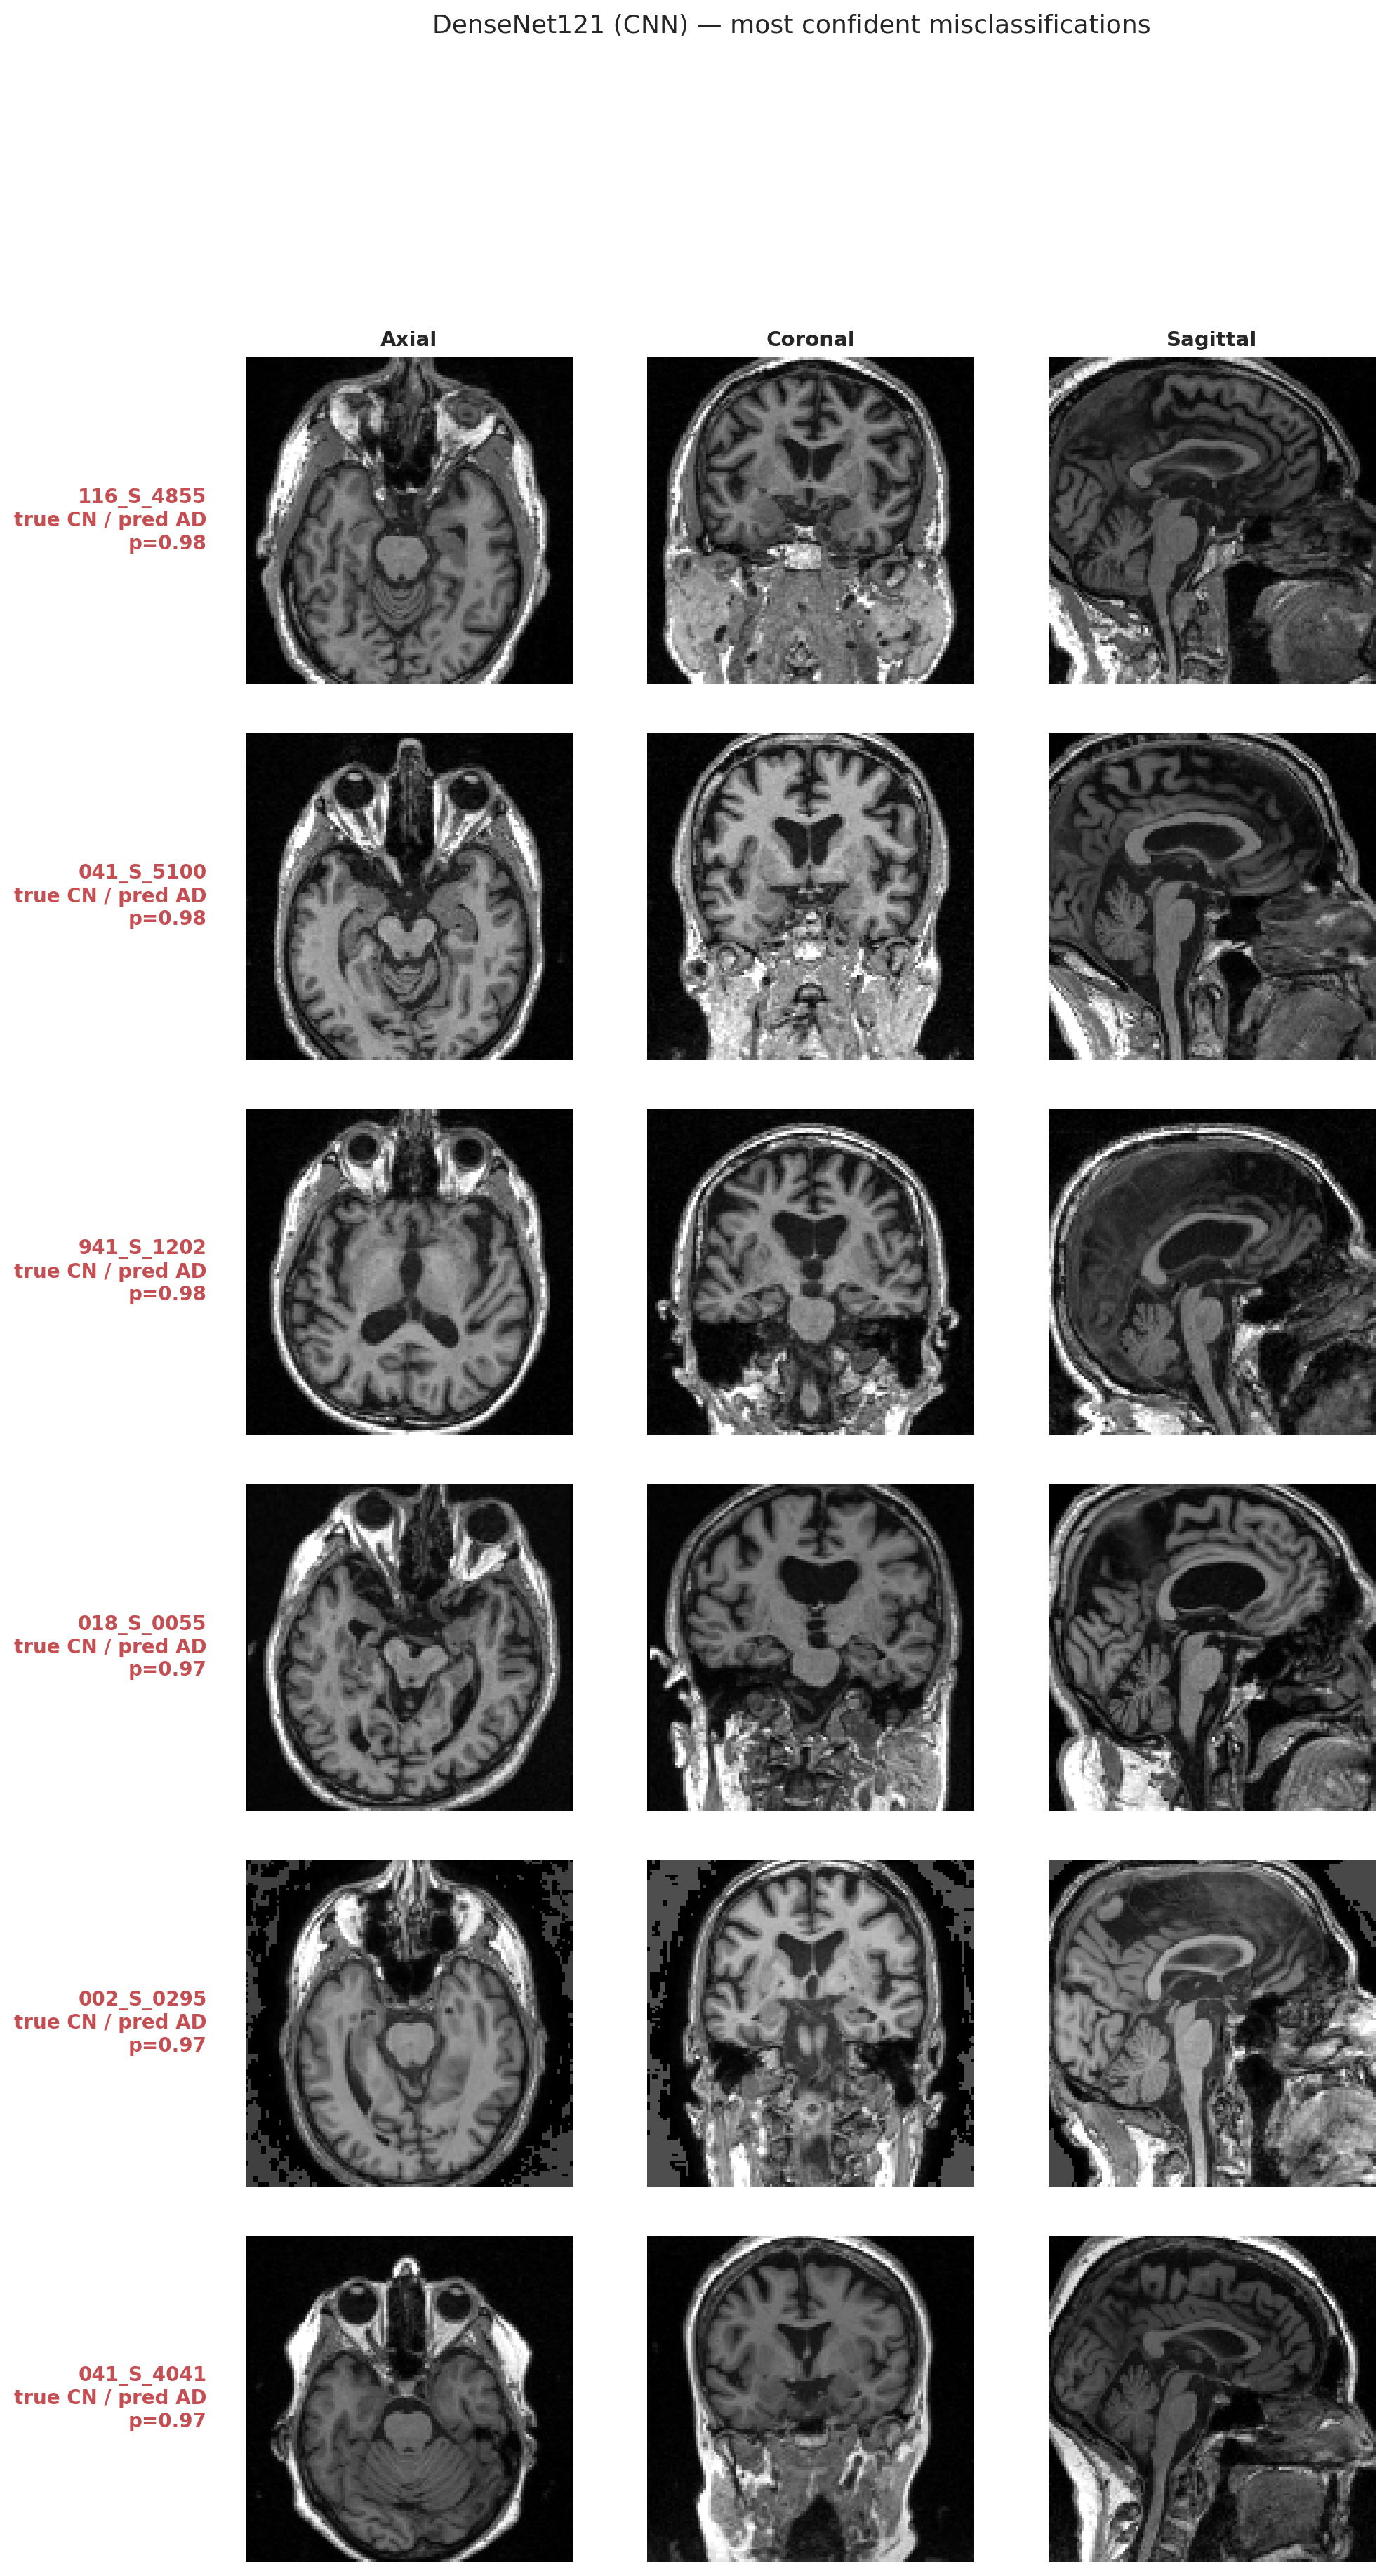
\includegraphics[width=7.6cm]{Images/err_binary_cnn_gallery.png}
    \caption[Error analysis (3 of 5 folds)]{\textbf{Error analysis (3 of 5 folds).} Binary predicted-probability histogram by true class (left) and a gallery of the most confident misclassifications (right) for the DenseNet CNN.}
    \label{fig:err}
\end{figure}

\section{Does the Hybrid Actually Help? (RQ1)}\label{sec:rq1}
The research question was whether fusing local (CNN) and global (transformer) 3D features beats either alone. The evidence is nuanced and reported honestly:
\begin{itemize}
    \item On the binary task the hybrid CNN--ViT has the highest mean, but its $+1.2$ accuracy / $+1.4$ macro-F1 margin over the standalone DenseNet is not statistically meaningful. The per-fold macro-F1 differences are $-0.052$, $+0.047$, $+0.065$, $-0.013$, and $+0.023$ (mean $+0.014$, SD $0.047$); a paired $t$-test gives $t=0.67$ with 4 degrees of freedom ($p\approx0.54$). The hybrid wins in only three of the five folds, and over all 315 subjects it classifies 259 correctly against the CNN's 255 --- a difference of four subjects.
    \item The result depends on \emph{which} branches are fused. CNN$+$ViT reaches $0.80$ macro-F1, whereas Swin$+$ViT, which has no convolutional branch, reaches $0.66$. This is consistent with the CNN branch carrying most of the signal at this data scale, but the comparison changes the first branch, not the fusion strategy, and no standalone ViT was run on the binary task, so the ViT branch's own contribution cannot be isolated.
\end{itemize}
The honest conclusion is that, on this dataset, \textbf{no improvement from hybridisation could be detected}: a well-trained 3D CNN is a very strong baseline, and adding a ViT branch leaves performance within fold-to-fold noise. A null result of this kind is a valid scientific finding, but a definitive answer to RQ1 would need standalone ViT and Swin runs on the binary task, a three-class CNN--ViT run, and repeated cross-validation with several seeds.

\section{Medical Transfer Learning: Pretrained ResNet vs. From-Scratch CNN}
Counter-intuitively, the MedicalNet-\emph{pretrained} 3D ResNet ($69.8\%$) was clearly \emph{worse} than the from-scratch DenseNet ($81.0\%$), and far less stable (std $0.139$ vs $0.041$). Our working hypothesis is that this is partly an \textbf{early-stopping artifact}. Its schedule makes a late take-off likely: the backbone is frozen for the first five epochs and then trained at a 10$\times$ lower learning rate ($10^{-5}$), while early stopping uses the shortest patience of any model (12 epochs). Three of the five folds are competitive while two stop before recovering. The two weak folds score an identical $0.449$, which is itself unusual and should be checked against the saved predictions. This hypothesis has not been tested here --- the per-fold ResNet curves are not shown, and the run was not repeated with a minimum-epoch guard before early stopping. The result should therefore be read as a property of the training schedule as much as of the architecture, not as evidence that medical pretraining is useless.

\section{Why the From-Scratch ViT Collapses}\label{sec:vit_collapse}
The pure 3D ViT reaches only $28.6\%$ on the three-class task, with almost no fold variance. This is not ``chance'' in the useful sense: it is far \emph{below} the $52.2\%$ obtained by always predicting the majority class. Its confusion matrix shows why --- the model \textbf{never predicts CN} and splits every subject between MCI and AD, and its training loss barely decreases. Two factors plausibly combine here. The first is the expected weakness of a data-hungry, low-inductive-bias transformer trained from scratch on a few hundred subjects, which is why the literature relies on large-scale pretraining for ViTs~\cite{dosovitskiy2021image}. The second is that the imbalance corrections (class weighting, weighted sampling, and focal loss) push a model that has learned nothing useful towards the minority classes; when several are active at once they can over-correct. Separating the two would require re-running the ViT with a single imbalance correction. Reported as a negative result, it supports pairing the transformer with a CNN, which supplies the missing inductive bias, rather than using a transformer alone.

\section{Explainability Analysis (RQ2)}
To test whether the models attend to anatomically meaningful regions, a suite of 3D attribution methods was applied (Grad-CAM, Grad-CAM++, Integrated Gradients, SmoothGrad, Occlusion, and attention rollout for the transformer branch)~\cite{selvaraju2017gradcam,sundararajan2017axiomatic,abnar2020quantifying}. Figure~\ref{fig:xai_panel} shows the method-comparison panel for the DenseNet CNN on one AD subject (\texttt{135\_S\_4863}, an axial slice at the level of the lateral ventricles). \textbf{The methods do not agree.} Grad-CAM highlights the frontal region; Grad-CAM++ and Score-CAM highlight a central, peri-ventricular area; occlusion responds mainly to the occipital region and the back of the skull; LIME includes part of the scalp; and Integrated Gradients is nearly empty on this slice.

\begin{figure}[H]
    \centering
    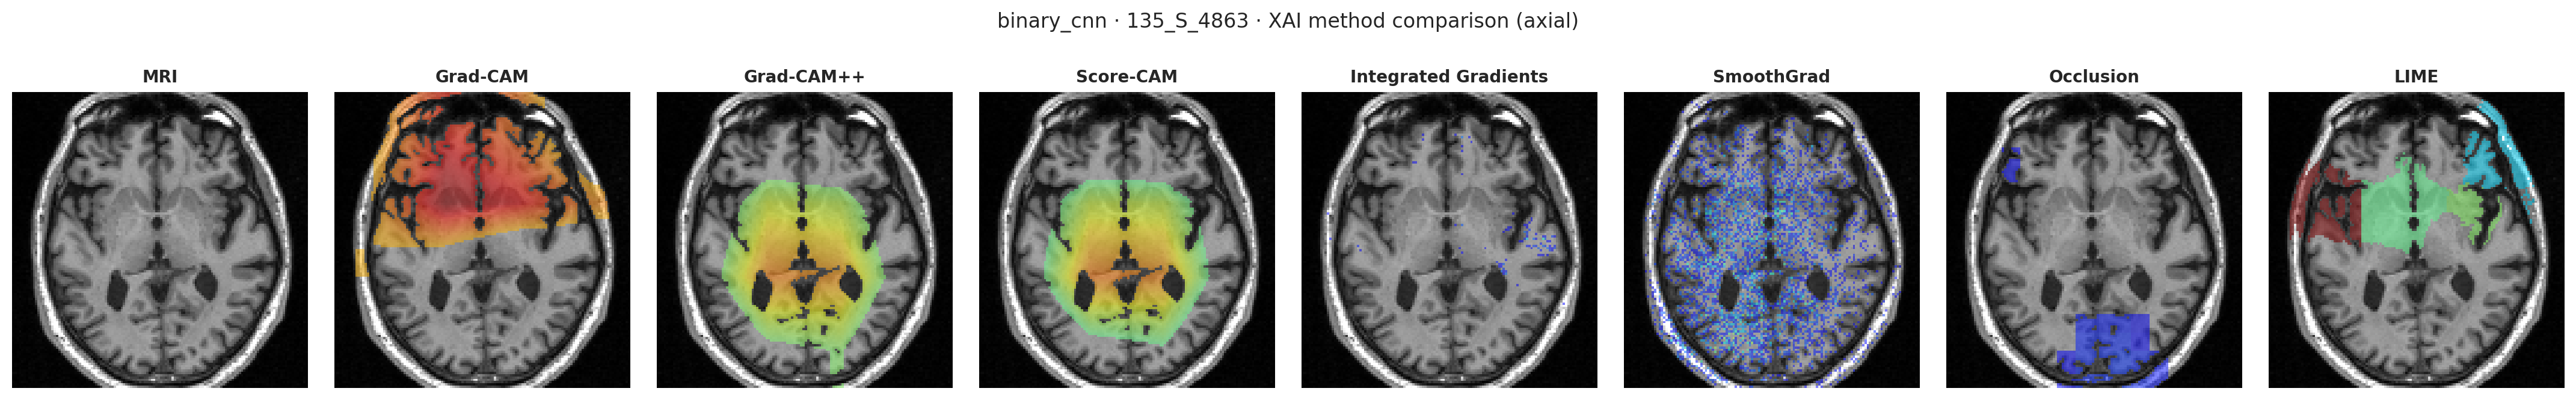
\includegraphics[width=15cm]{Images/xai_panel_binary_cnn.png}
    \caption[XAI method comparison]{\textbf{XAI method comparison.} Explainability for the binary DenseNet CNN on one AD subject: Grad-CAM, Grad-CAM++, Score-CAM, Integrated Gradients, SmoothGrad, Occlusion, and LIME. The methods highlight different regions, including non-brain tissue.}
    \label{fig:xai_panel}
\end{figure}

Because the hybrid CNN--ViT checkpoints were not retained, \textbf{no explanation maps exist for the proposed model}; the per-subject maps above use the standalone DenseNet, which is statistically tied with it. The group-level regional analysis (Figure~\ref{fig:xai_roi}) was computed for a different model, the binary \emph{Swin--ViT} hybrid, over 16 AD subjects from a single fold. It splits the volume into thirds along each axis. The result is close to uniform (all nine values lie between $0.036$ and $0.055$): on the left--right axis the \emph{middle} third is the \emph{lowest}, and the posterior and inferior thirds receive slightly more importance than the anterior and superior thirds. This does not show a concentration on medial or central structures.

\begin{figure}[H]
    \centering
    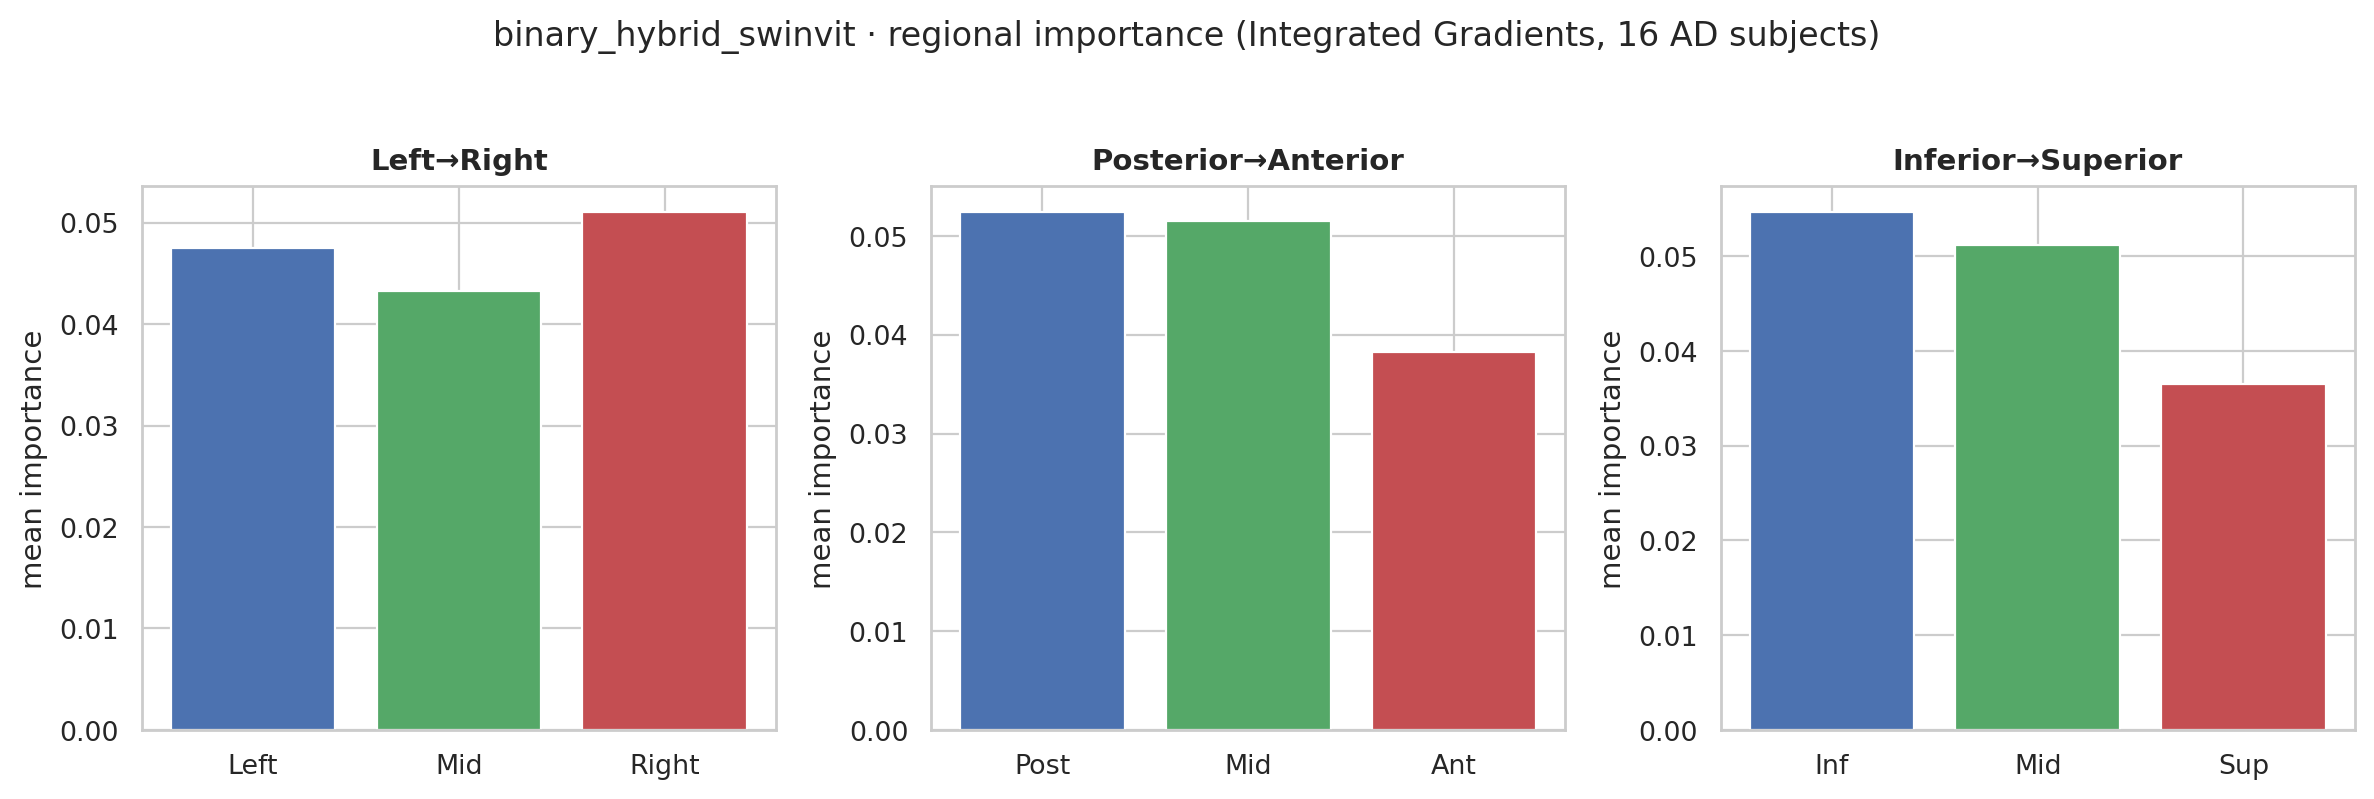
\includegraphics[width=13cm]{Images/xai_roi_binary.png}
    \caption[Group-averaged importance (Swin--ViT)]{\textbf{Group-averaged importance (Swin--ViT hybrid, 16 AD subjects, one fold).} Mean Integrated-Gradients importance over spatial thirds of the head volume. \textbf{Honesty note:} the ADNI volumes are not skull-stripped or atlas-registered, so these are coarse thirds of the head volume, not anatomical ROIs.}
    \label{fig:xai_roi}
\end{figure}

Taken together, these maps do \emph{not} yet establish that the models rely on AD-relevant anatomy. Because the skull, scalp, orbits, and neck are still present in the input, a model could exploit non-brain cues, and several methods do place importance there. Establishing anatomical grounding would require skull-stripping, registration to an atlas so that importance can be summed over named ROIs such as the hippocampus, and sanity checks such as model-randomisation tests and deletion curves.

Figure~\ref{fig:xai_hybrid} shows the panel for the Swin--ViT hybrid, including \textbf{attention rollout} from the transformer branch. On this inferior slice, attention rollout falls near the orbit and skull base, Grad-CAM falls largely on the scalp and posterior neck, and occlusion highlights the cerebellum. Figure~\ref{fig:xai_3class} shows the three-class Swin panel and its group-averaged Integrated Gradients over 16 correctly classified AD subjects. The per-subject Grad-CAM again responds to extra-cerebral tissue (temporal muscle and orbits) as well as the cerebellum, and the group-averaged attribution is diffuse --- spread across the cortex, cerebellum, brainstem, and scalp rather than focused on the medial temporal lobe. These maps are reported for transparency; they are not evidence of disease-specific localisation.

\begin{figure}[H]
    \centering
    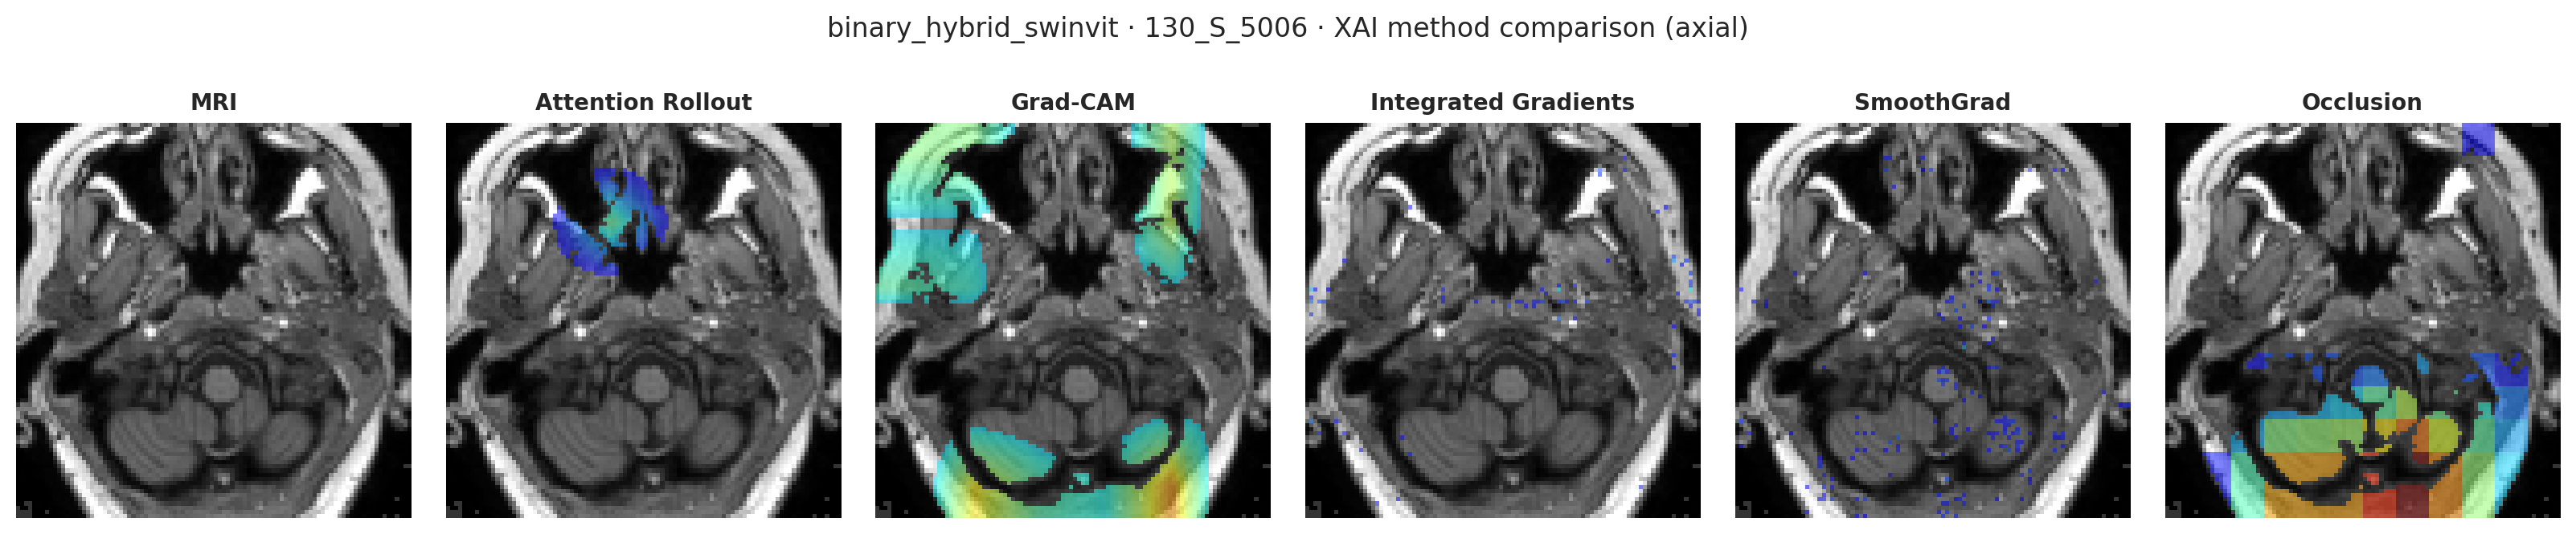
\includegraphics[width=15cm]{Images/xai_panel_hybrid.png}
    \caption[Swin--ViT hybrid explainability]{\textbf{Swin--ViT hybrid explainability.} Panel for the binary Swin--ViT hybrid (not the proposed CNN--ViT), including transformer attention rollout alongside Grad-CAM, Integrated Gradients, SmoothGrad, and occlusion.}
    \label{fig:xai_hybrid}
\end{figure}

\begin{figure}[H]
    \centering
    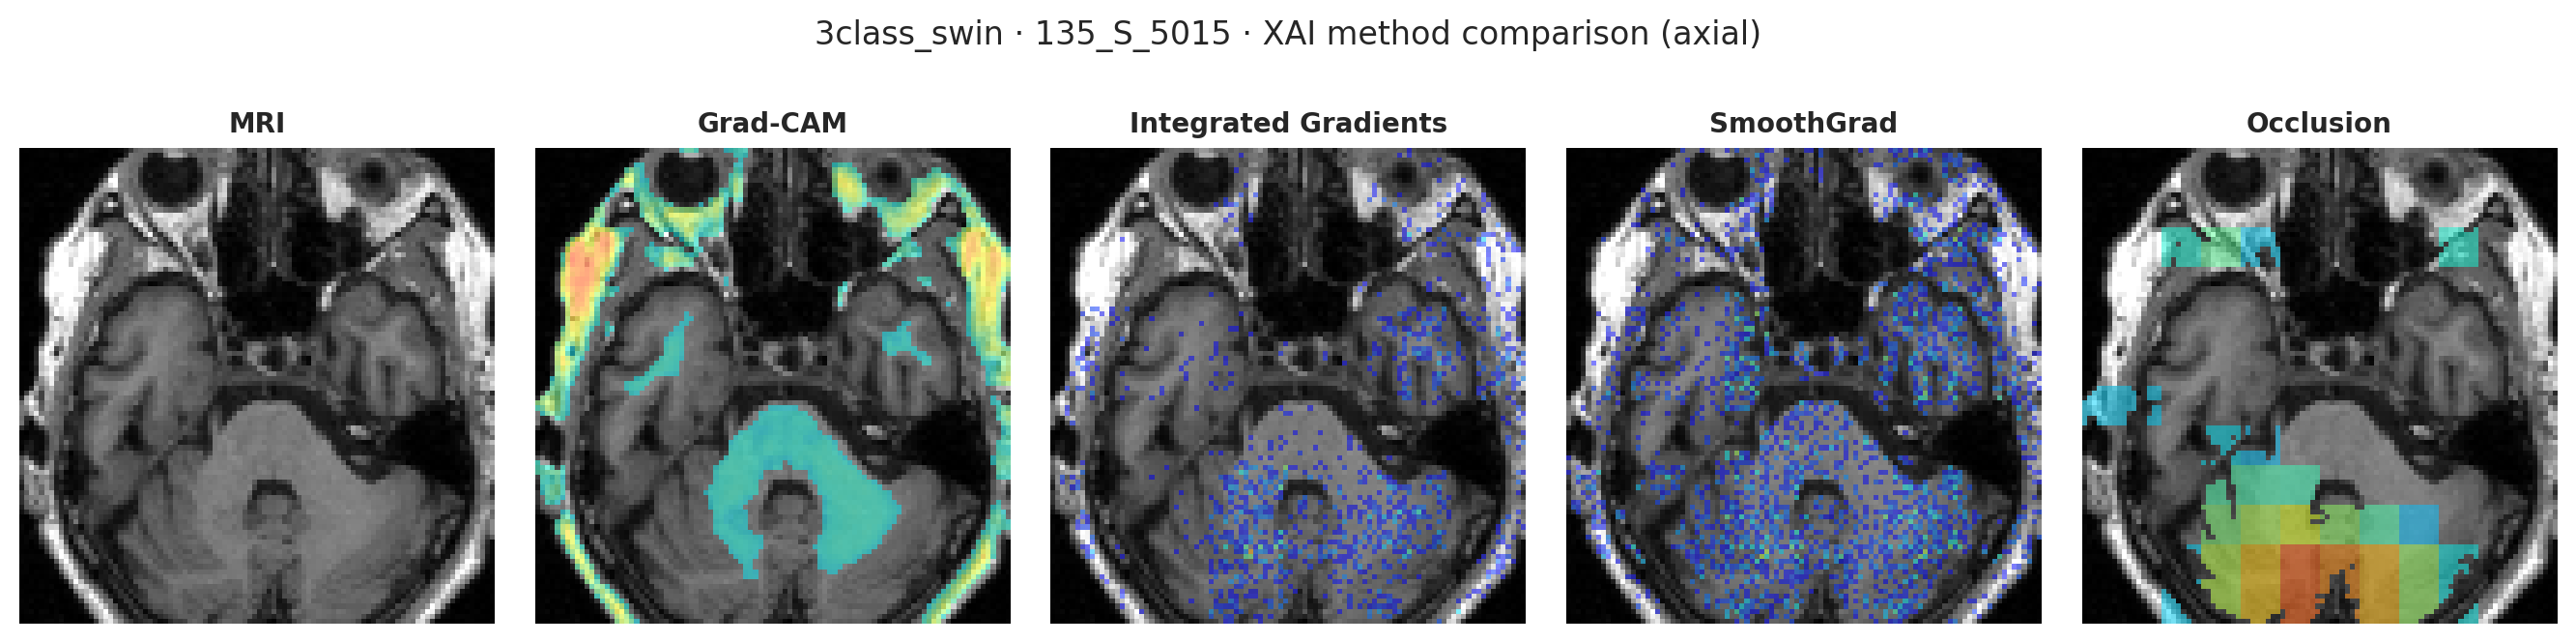
\includegraphics[width=10.5cm]{Images/xai_panel_3class_swin.png}\\[4pt]
    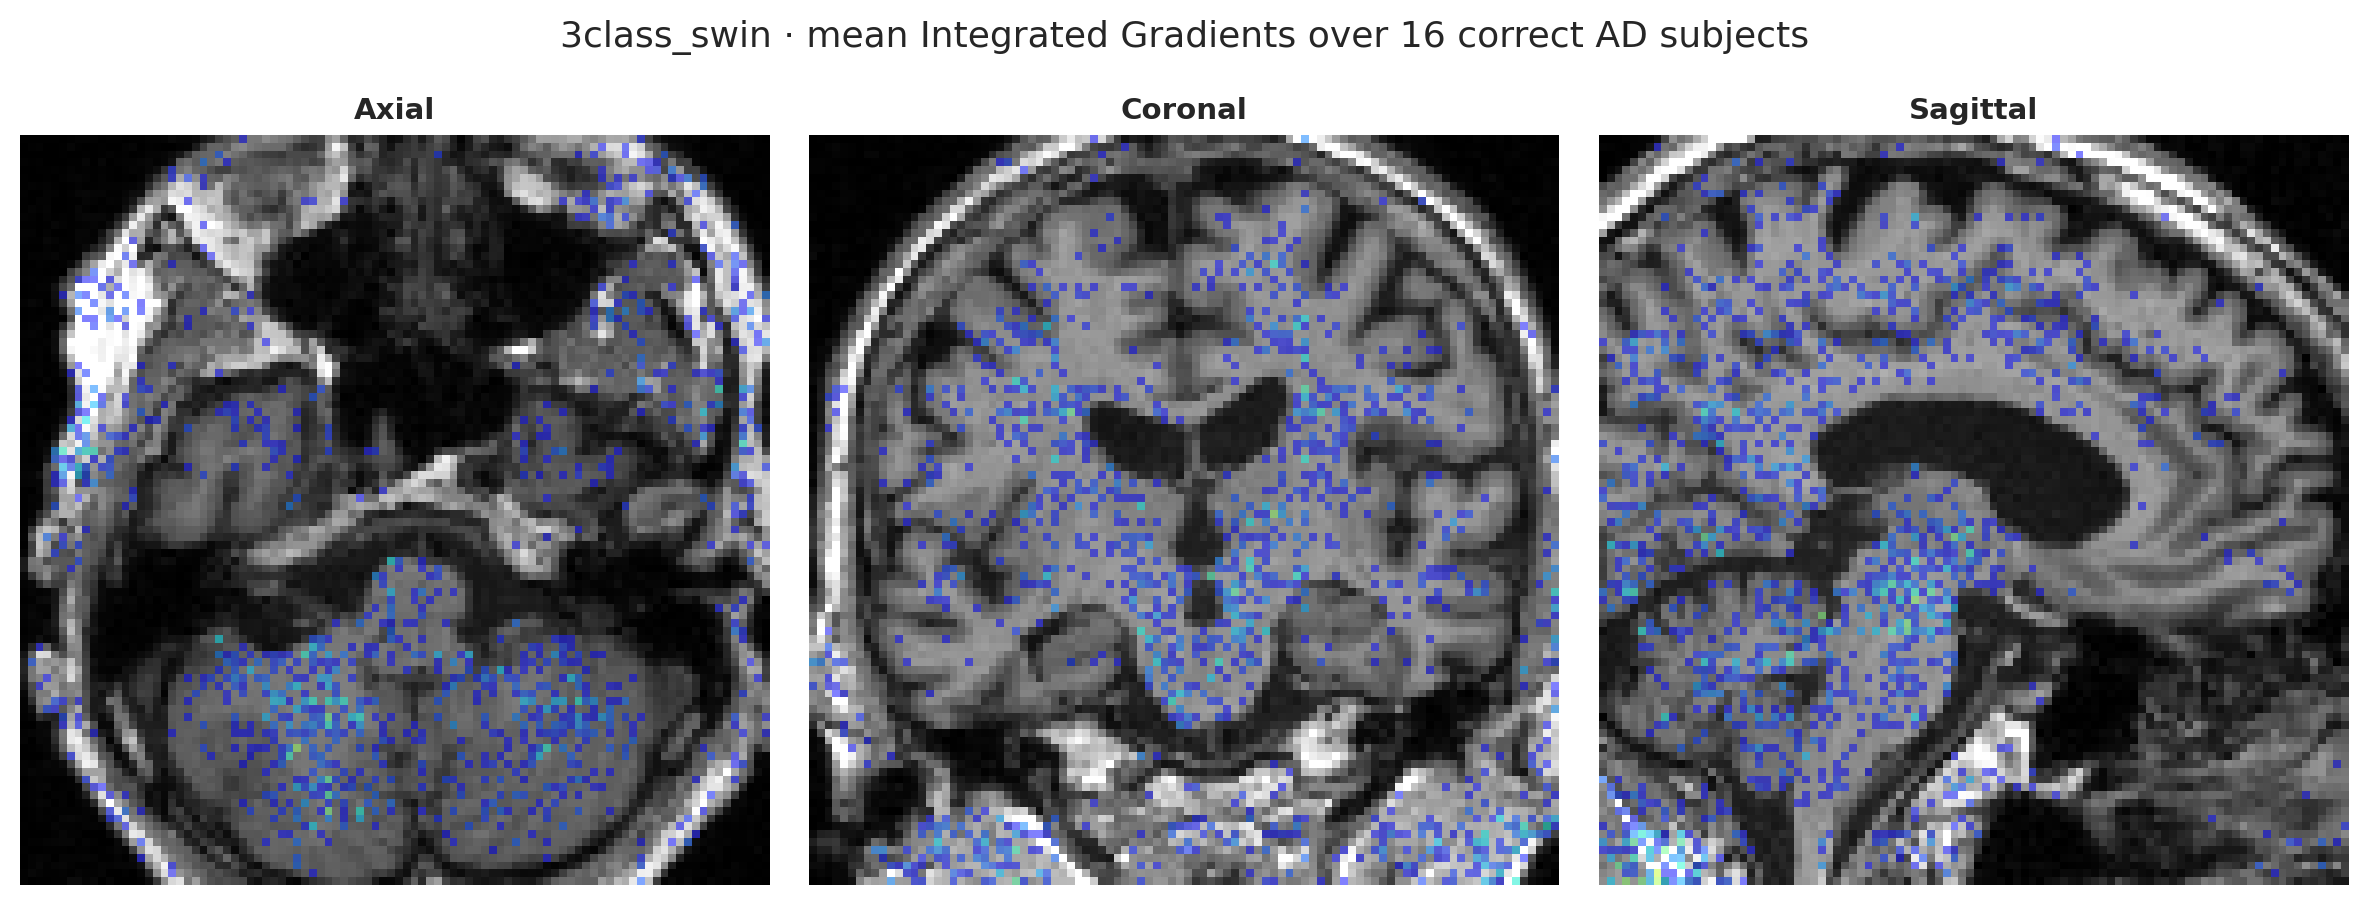
\includegraphics[width=12cm]{Images/xai_groupavg_3class.png}
    \caption[Three-class explainability]{\textbf{Three-class explainability.} Swin per-subject method panel (top) and group-averaged Integrated-Gradients importance (bottom).}
    \label{fig:xai_3class}
\end{figure}

\section{Comparison with the Literature}
Table~\ref{tab:compare_lit} places these results against the accuracies surveyed in Chapter~\ref{cha:LiteratureReviewU}. Many reported systems exceed $98\%$, but almost all split the data at the level of 2D slices (or use the curated Kaggle 2D set), which leaks a patient's slices across train and test and inflates accuracy~\cite{wen2020convolutional,yagis2021effect}. Studies that evaluate whole 3D volumes at the subject level report far more modest numbers: Wen \etal~\cite{wen2020convolutional} obtain $85$--$88\%$ for AD-vs-CN with subject-level 3D CNNs, and the ROI-based 3D ViT ensemble~\cite{saoud2024explainable}, which uses one baseline scan per subject, reports $90\%$ for AD-vs-CN and only $60\%$ for three-class. This work's $82\%$ (binary) and $58\%$ (three-class, Swin) lie in the same regime, but somewhat \emph{below} these subject-level references. The gap is plausibly explained by the absence of skull-stripping and registration, the reduced $96^3$ input resolution, and the small cohort. The numbers here should therefore be read as \emph{trustworthy} rather than state-of-the-art.

\begin{table}[H]
\centering
\caption{This work vs.\ reported literature, highlighting the evaluation protocol.}
\label{tab:compare_lit}
\begin{tabular}{|p{5.2cm}|p{2.6cm}|p{2.6cm}|p{2.6cm}|}
\hline
\textbf{Study / Model} & \textbf{Split level} & \textbf{Binary AD-CN} & \textbf{3-class} \\
\hline
Slice-based ViT / CNN studies~\cite{alsaeed2022brain,mahim2024unlocking,alshayeji2024alzheimer,el2024novel} & 2D slice (leakage-prone) & 98--99\% & 99\% \\
Subject-level 3D CNNs~\cite{wen2020convolutional} & subject & 85--88\% & --- \\
ROI 3D ViT ensemble~\cite{saoud2024explainable} & subject (1 baseline scan per subject, ROI) & 90\% & 60\% \\
\textbf{This work} & \textbf{subject-level} & \textbf{82.2\%} (CNN--ViT) & \textbf{57.7\%} (Swin) \\
\hline
\end{tabular}
\end{table}

\section{Answers to the Research Questions}
The evidence gathered above answers the two research questions posed in Chapter~\ref{cha:introduction} directly.

\noindent\textbf{RQ1 --- Does fusing local (CNN) and global (ViT) features improve accuracy?} \emph{No improvement was detected.} The hybrid CNN--ViT has the highest binary mean ($82.2\%$ / macro-F1 $0.802$), but it is statistically indistinguishable from the from-scratch DenseNet ($81.0\%$ / $0.788$; paired $p\approx0.54$, three of five folds won). The configuration without a CNN branch (Swin--ViT) is clearly weaker, which suggests that the CNN carries most of the signal. The question is only partly answered: standalone ViT and Swin models were not run on the binary task, and the hybrid was not run on the three-class task.

\noindent\textbf{RQ2 --- Can 3D explainability give clinically meaningful explanations?} \emph{Not yet demonstrated.} The 3D attribution pipeline works end-to-end and produces maps for the CNN, Swin, and Swin--ViT models (Figures~\ref{fig:xai_panel}--\ref{fig:xai_3class}). However, the methods disagree on individual subjects, several of them assign importance to non-brain tissue, and the group-level regional analysis is close to uniform. No maps exist for the proposed CNN--ViT. Because the volumes are not skull-stripped or atlas-registered, the current evidence cannot distinguish disease-related anatomy from other cues; Chapter~\ref{cha:ConclusionAndFutureWork} lists the steps needed to answer RQ2 properly.

\section{Threats to Validity}
Several factors bound the strength of these conclusions and are stated openly. \textbf{Sample size:} 395 subjects (only 80 MCI) is small, so the three-class estimates in particular carry wide fold-to-fold variance. \textbf{Single cohort:} ADNI is itself multi-site and multi-scanner, but using it alone leaves generalisation to other cohorts, populations, and acquisition protocols untested. \textbf{Incomplete grid:} standalone ViT and Swin were not run on the binary task, and the proposed CNN--ViT was not run on the three-class task, so RQ1 is only partly answered. \textbf{Statistical power:} with a single seed and five folds, differences of one or two points cannot be distinguished from noise. \textbf{Partial diagnostics:} the binary CNN's ROC, calibration, and error-analysis figures cover three of the five folds. \textbf{Demographics:} the groups are age- and sex-matched, and a class-balanced logistic regression on age and sex alone, trained on the same folds, stays at chance (binary balanced accuracy $0.50$, AUC $0.48$; three-class balanced accuracy $0.38$), so the models' signal is not explained by demographics. \textbf{Unequal recipes:} the schedules and input sizes differ between some models (Appendix~\ref{app:repro}), so model comparisons are between tuned configurations rather than single-factor ablations. \textbf{Training-schedule confound:} the pretrained-ResNet result is partly an early-stopping artifact rather than a pure architecture effect. \textbf{Explainability:} without skull-stripping or registration, importance is reported over coarse spatial regions rather than atlas ROIs, the methods disagree, and maps were computed for models other than the proposed hybrid. Each of these marks a place where stronger claims would need the additional work outlined in Chapter~\ref{cha:ConclusionAndFutureWork}.

\section{Summary}
On a leakage-free, subject-level ADNI benchmark, the proposed hybrid 3D CNN--ViT has the highest binary CN-vs-AD mean ($82.2\%$, macro-F1 $0.80$) but is statistically tied with a strong from-scratch DenseNet. The three-class result is an honest $\sim\!57\%$ (Swin), only about five points above the majority-class baseline and bottlenecked by MCI. Medical transfer learning (pretrained ResNet) underperformed, partly due to an early-stopping artifact, and a from-scratch ViT failed outright --- both reported as instructive negative results. The explainability maps are inconsistent across methods and include non-brain regions, so they do not yet support anatomical conclusions. Together these results answer the two research questions as follows: no benefit from hybridisation could be detected (RQ1, partly answered), and anatomically grounded explanation is not yet demonstrated (RQ2).
